\documentclass[17pt, a0paper, portrait, margin=0mm, innermargin=5mm, blockverticalspace=7mm, colspace=6.5mm, subcolspace=6.5mm]{tikzposter}

% comment: screenshot plaatjes max 15cm als fullscreen screenshot

\tikzposterlatexaffectionproofoff

% \title{\parbox{\linewidth}{\centering Estimating drawdown using time series analysis}}
\title{\parbox{\linewidth}{\centering Going off-grid locally: Coupling analytic elements with finite difference models}}
\author{Davíd A. Brakenhoff$\,^{1,2}$, Mark Bakker$\,^2$}
\institute{$^1\,$Artesia B.V. $^2\,$Delft University of Technology}

% kleurcode Modflow and More logo: 00234B, omgezet naar 065887 (comp 004798)
% colorthemes
% IAH: 116699, cccccc, c3312f
% https://colorhunt.co/palette/
% 07689fa2d5f2fafafaff7e67: FF7E67, A2D5F2, 07689F
% martin: FF7E67, A2D5F2, , F2BFA2 (comp. A2D5F2)

% define colors in HEX code (https://colorhunt.co/palette/07689fa2d5f2fafafaff7e67)
% \newcommand{\colorTitle}{07689F}            % title block main color
% \newcommand{\colorTitleGradient}{07689F}    % title block gradient color
% \newcommand{\colorBlockTitle}{d97669}       % color of block title
% \newcommand{\colorBlock}{ffe2dd}            % color of blocks
\newcommand{\colorBlockTitleText}{FFFFFF}   % color of block title text

% define colors in HEX code (https://colorhunt.co/palette/e7e6e1f7f6e7f2a154314e52)
% \newcommand{\colorTitle}{314E52}            % title block main color
% \newcommand{\colorTitleGradient}{314E52}    % title block gradient color
% \newcommand{\colorBlockTitle}{F2A154}       % color of block title
% \newcommand{\colorBlock}{F7F6E7}            % color of blocks
% \newcommand{\colorBlockTitleText}{FFFFFF}   % color of block title text

% define colors in HEX code (https://colorhunt.co/palette/062c3005595be2d784f5f5f5)
% \newcommand{\colorTitle}{05595B}            % title block main color
% \newcommand{\colorTitleGradient}{05595B}    % title block gradient color
% \newcommand{\colorBlockTitle}{E2D784}       % color of block title
% \newcommand{\colorBlock}{F5F5F5}            % color of blocks
% \newcommand{\colorBlockTitleText}{FFFFFF}   % color of block title text

% define colors in HEX code (https://colorhunt.co/palette/feece9ccd1e4fe7e6d2f3a8f)
% \newcommand{\colorTitle}{2F3A8F}            % title block main color
% \newcommand{\colorTitleGradient}{2F3A8F}    % title block gradient color
% \newcommand{\colorBlockTitle}{FE7E6D}       % color of block title
% \newcommand{\colorBlock}{FEECE9}            % color of blocks
% \newcommand{\colorBlockTitleText}{062C30}   % color of block title text

% define colors in HEX code
% \newcommand{\colorTitle}{1A5319}            % title block main color, cobalt
% \newcommand{\colorTitleGradient}{1A5319}    % title block gradient color, cobalt
% % \newcommand{\colorTitle}{921224}            % title block main color, darkred
% % \newcommand{\colorTitleGradient}{921224}    % title block gradient color, darkred
% \newcommand{\colorBlockTitle}{508D4E}       % color of block title
% \newcommand{\colorBlock}{FFFFFF}            % color of blocks
% \newcommand{\colorBlockTitleText}{062C30}   % color of block title text

% define colors in HEX code (current fave)
\newcommand{\colorTitle}{003C43}            % title block main color, cobalt
\newcommand{\colorTitleGradient}{003C43}    % title block gradient color, cobalt
% \newcommand{\colorTitle}{921224}            % title block main color, darkred
% \newcommand{\colorTitleGradient}{921224}    % title block gradient color, darkred
% \newcommand{\colorBlockTitle}{0B666A}       % color of block title
\newcommand{\colorBlockTitle}{0c6f73}       % color of block title
\newcommand{\colorBlock}{FFFFFF}            % color of blocks
% \newcommand{\colorBlockTitleText}{062C30}   % color of block title text


% % define colors in HEX code (gekke optie)
% \newcommand{\colorTitle}{1230AE}            % title block main color, cobalt
% \newcommand{\colorTitleGradient}{1230AE}    % title block gradient color, cobalt
% % \newcommand{\colorTitle}{921224}            % title block main color, darkred
% % \newcommand{\colorTitleGradient}{921224}    % title block gradient color, darkred
% % \newcommand{\colorBlockTitle}{0B666A}       % color of block title
% \newcommand{\colorBlockTitle}{6C48C5}       % color of block title
% \newcommand{\colorBlock}{FFFFFF}            % color of blocks
% % \newcommand{\colorBlockTitleText}{062C30}   % color of block title text

\definecolor{colorBlockTitle}{HTML}{0c6f73}

% new color definitions for Desert theme
\definecolorpalette{GrayOrangeBlue}{
    \definecolor{colorOne}{HTML}{\colorTitle} %bovenkant
    \definecolor{colorTwo}{HTML}{\colorBlock} %tekstvakken
    \definecolor{colorThree}{HTML}{\colorBlockTitle} %tekstkoppen
}
% bottom color for title block and top color for lower block
\definecolor{gradientcolor}{HTML}{\colorTitleGradient}

% Remove gradient in title block
\definetitlestyle{VerticalShading}{
	width=\paperwidth, roundedcorners=0, linewidth=0pt, innersep=1.5cm,
	titletotopverticalspace=0mm, titletoblockverticalspace=20mm,
	titlegraphictotitledistance=10pt, titletextscale=1
}{
   \draw[draw=none, bottom color=gradientcolor, top color=colorOne]%
   (\titleposleft,\titleposbottom) rectangle (\titleposright,\titlepostop);
}
% remove gradient in bottom (modify top color=...)
\definebackgroundstyle{BottomVerticalGradation}{
	\draw[draw=none, line width=0pt, bottom color=colorOne, 
	    top color=gradientcolor] (bottomleft) rectangle ($(bottomleft)+(\textwidth,2.5)$); 
}

% remove gradient in text block titles (modify right color=...)
\defineblockstyle{Slide}{
	titlewidthscale=1, bodywidthscale=1, titleleft,
	titleoffsetx=0pt, titleoffsety=0pt, bodyoffsetx=0pt, bodyoffsety=0pt,
	bodyverticalshift=0pt, roundedcorners=0, linewidth=0pt, titleinnersep=1cm,
	bodyinnersep=1cm 
}{
	\ifBlockHasTitle%
		\draw[draw=none, left color=colorThree, right color=colorThree]
		   (blocktitle.south west) rectangle (blocktitle.north east);
	\fi%
	\draw[draw=none, fill=blockbodybgcolor] %
		(blockbody.north west) [rounded corners=15] -- (blockbody.south west) --
		(blockbody.south east) [rounded corners=0]-- (blockbody.north east) -- cycle;
}
% Turn off gray gradient in title and bottom bar
\definecolorstyle{sampleColorStyle} {
    \definecolor{colorOne}{HTML}{\colorTitle} %bovenkant
    \definecolor{colorTwo}{HTML}{\colorBlock} %tekstvakken
    \definecolor{colorThree}{HTML}{\colorBlockTitle} %tekstkoppen
    \definecolor{gradientcolor}{HTML}{\colorTitleGradient}
    \definecolor{blocktitlefgcolor}{HTML}{\colorBlockTitleText}
}{
%     % Background Colors
    \colorlet{backgroundcolor}{white}
    \colorlet{framecolor}{colorOne}
%     % Title Colors
    \colorlet{titlefgcolor}{white}
    \colorlet{titlebgcolor}{gradientcolor}
%     % Block Colors
    % \colorlet{blocktitlebgcolor}{white}
    \colorlet{blocktitlefgcolor}{blocktitlefgcolor}
    % \colorlet{blockbodybgcolor}{white}
    % \colorlet{blockbodyfgcolor}{white}
}

\usetheme{Desert} % uses edited colorpalatte if GrayOrangeBlue
\usebackgroundstyle{Filled}
\usetitlestyle{VerticalShading}  % use Filled and change \colorTitleGradient to avoid gradient?
\usecolorstyle[colorPalette=GrayOrangeBlue]{sampleColorStyle}

\makeatletter
\renewcommand\TP@maketitle{\centering
\begin{minipage}[c][][t]{175mm}
    
\includegraphics[width=80mm]{logo/logo_artesia.png}
    \hfill
    % \includesvg[width=80mm]{logo/logo_tud.svg}
    
\includegraphics[width=80mm]{logo/logo_tudelft.png}
\end{minipage}
\hfill
\begin{minipage}[c][][c]{475mm}
    \centering
    \color{titlefgcolor}
    {\bfseries \Huge \sc \sffamily \@title \par}
    \vspace*{5mm}
    {\LARGE \sc \sffamily \@author \par}
    \vspace*{5mm}
    {\Large \sffamily \@institute \par}
\end{minipage}
\hfill
\begin{minipage}[c][][t]{150mm}
    \centering
    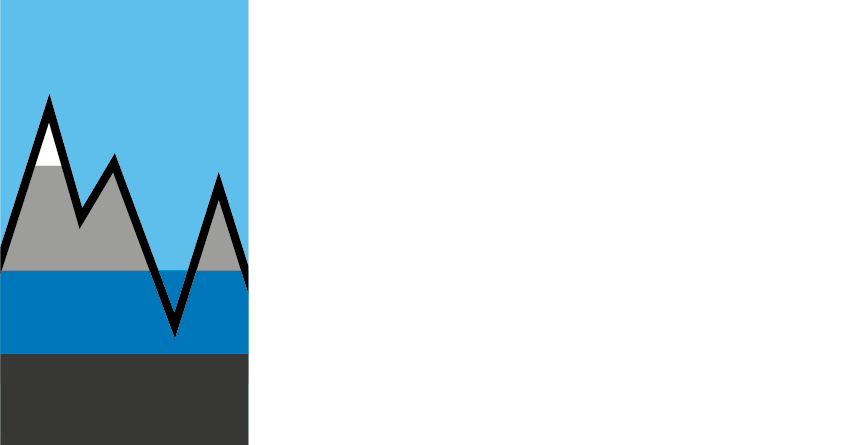
\includegraphics[width=90mm]{logo/logo_iah.png}
\end{minipage}

}%
\makeatother

\usepackage[square, sort, numbers]{natbib}
\bibliographystyle{unsrtnat}
\usepackage{svg}
\usepackage{booktabs}
\usepackage{multicol}
\setlength{\columnsep}{10mm}

\usepackage{xpatch}
\xpatchcmd{\block}{\bf\LARGE\color{blocktitlefgcolor}}{\sffamily\bfseries\LARGE\color{blocktitlefgcolor}}{}{}

\usepackage{xcolor}

 % Subcolumns environment
\makeatletter
\newenvironment{subcolumns}{
    \ifTP@columnEnvironment
        \TP@subcolumnEnvironmenttrue
        \setlength{\TP@subcolcenter}{\TP@colcenter-0.5\colwidth-\TP@subcolspace}
        \global\TP@subcolcenter=\TP@subcolcenter
        \global\TP@subcoltop=\TP@blocktop
        \global\TP@subcolbottom=\TP@blocktop
        \subcolwidth=0pt
    \fi
}{
    \TP@subcolumnEnvironmentfalse
    \global\TP@blocktop=\TP@subcolbottom
}

 % Subcolumn
\gdef\subcolumn#1{  % #1: relative width
    \ifTP@subcolumnEnvironment
        \normalsize
        \setlength{\TP@blocktop}{\TP@subcoltop}
        \setlength{\TP@subcolcenter}{\TP@subcolcenter+0.5\subcolwidth+\TP@subcolspace}
        \setlength{\subcolwidth}{#1\colwidth+#1\TP@subcolspace-\TP@subcolspace}
        \setlength{\TP@subcolcenter}{\TP@subcolcenter+0.5\subcolwidth}
    \fi
}
\makeatother

\makeatletter
\renewenvironment{tikzfigure}[1][]{
  \def \rememberparameter{#1}
  \vspace{6pt}
  \refstepcounter{figurecounter}
  \begin{center}
  }{
    \ifx\rememberparameter\@empty
    \else %nothing
    \\[7pt]
    {\RaggedRight \small Fig.~\thefigurecounter: \rememberparameter}
    \fi 
  \end{center}
}
\makeatother

\makeatletter
\newcounter{tablecounter}
\newenvironment{tikztable}[1][]{
  \def \rememberparameter{#1}
  \vspace{10pt}
  \refstepcounter{tablecounter}
  \begin{center}
  }{
    \ifx\rememberparameter\@empty
    \else
    \\[15pt]
    {\RaggedRight \small Tab.~\thetablecounter: \rememberparameter}
    \fi
  \end{center}
}
\makeatother

\usepackage[square, sort, numbers]{natbib}
\bibliographystyle{unsrtnat}
\usepackage{svg}
\usepackage{booktabs}
\usepackage{multicol}
\setlength{\columnsep}{10mm}
\usepackage[font=small,skip=-2pt]{caption}
\usepackage{graphics}
\usepackage{vwcol}
\usepackage{fontawesome5}
\usepackage{color,soul}
\usepackage{enumitem}
\usepackage{amsmath}

\renewcommand*{\emailsymbol}{{\small\faIcon[solid]{envelope}}~} % alternative: \faInbox

% tikz for flowchart
\usepackage{tikz}
\usetikzlibrary{shapes.geometric, arrows, positioning, fit}
\tikzstyle{io} = [trapezium, trapezium left angle=80, trapezium right angle=100, text width=7.5cm, minimum height=1cm, text centered, draw=black]
\tikzstyle{process} = [rectangle, text width=11cm, minimum height=1cm, text centered, draw=black]
\tikzstyle{select} = [rectangle, text width=11cm, minimum height=1cm, text centered, draw=black, rounded corners]
\tikzstyle{arrow} = [thick,->,>=stealth]

\begin{document}

\maketitle

\begin{columns}
\column{0.5}
% Introduction
  \block[bodyoffsety=5mm,titleoffsety=5mm,bodyverticalshift=-5mm]{Introduction}{
    \begin{multicols}{2}
    
        The analytic element method (AEM) is a gridless technique for modeling groundwater flow problems in which each feature that affects groundwater flow is described using an analytical solution. Superposition of these solutions can be used to gain insight into complex geohydrological problems. The advantages of AEM are that no spatial or temporal discretization is required and that the locations of elements are exact. The head can be computed at any location and at any time within the model domain. One disadvantage is that the computation of the head requires computing the contribution of each element in the model, causing models with many elements to become somewhat computationally intensive. Though computational solutions exist to mitigate these downsides, finite difference (FD) groundwater models such as Modflow 6 are highly efficient and capable of modeling large-scale heterogeneous groundwater flow problems. However, these numerical groundwater models require both temporal and spatial discretization. This requires the modeler to make choices that fit the problem. In mixed-scale problems, e.g. local head changes in a large aquifer system, trade-offs between computation time and level of detail have to be considered.
        
        \vspace{3mm}

        % In this fashion, a block of finite difference cells is replaced by an AEM model. Both models are solved simultaneously, which satisfies the water balance. Specially developed analytic line-elements facilitate the communication between the two models. Benchmark problems showcase the accuracy of the implementation and the challenges that arise from coupling numerical and analytic models.
    
    \end{multicols}

    \vspace{5mm}

    \centering
    \setulcolor{colorBlockTitle}
    \bf{\ul{\Large The goal of this research is to tightly couple an analytic element model to a finite difference model.}}
    
}

    \block[bodyverticalshift=-8mm]{Analytic Model of a Finite Difference Cell}{

        \begin{multicols}{3}

        The coupling of FD and AEM is demonstrated by replacing one cell in the FD model with an analytic element model. An analytic element model of that cell requires the following elements:

        \vspace{3mm}
        
        \begin{itemize}[noitemsep]
            \item boundary elements to control the fluxes in/out of the AEM model
            \item any internal elements that affect groundwater flow (e.g. wells)
            \item and a constant
        \end{itemize}

        \vspace{3mm}
        
        Solving these models simultaneously requires communication between the two models such that the water balance is met.

        \begin{tikzfigure}[FD model where the middle cell is replaced by an AEM model.\par]
            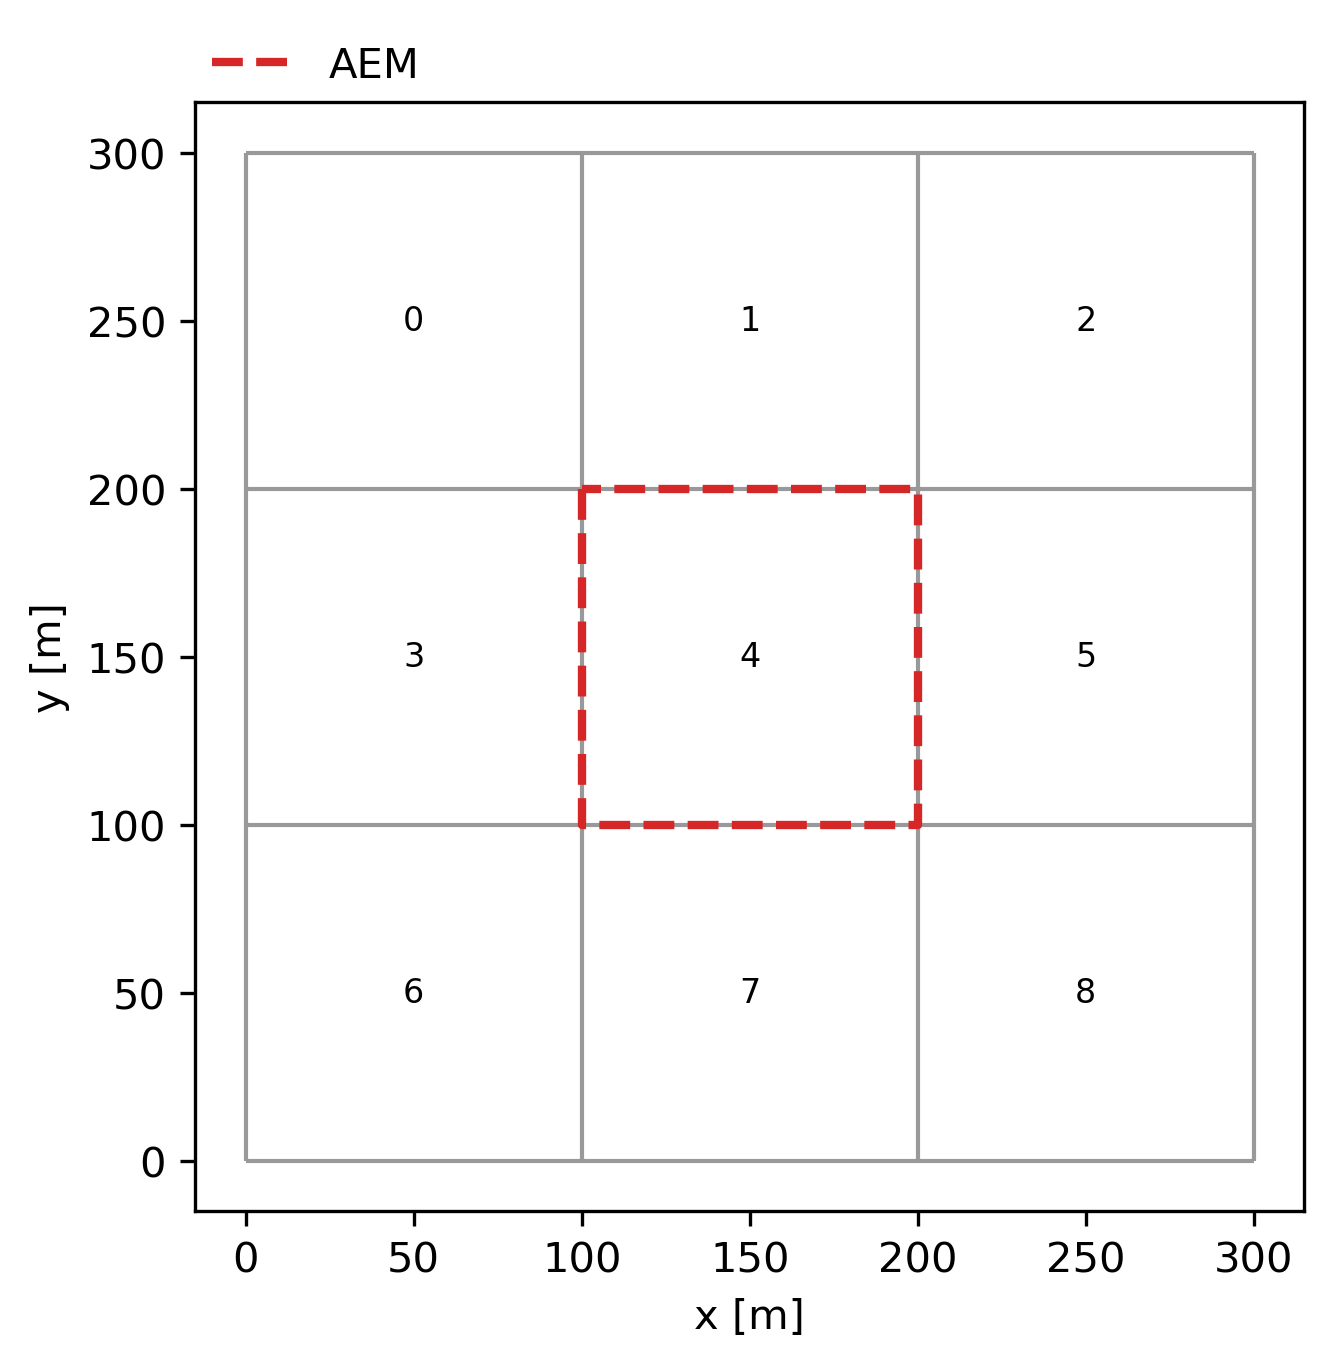
\includegraphics[height=100mm]{figures/test_model.png}
        \end{tikzfigure}
        
        \begin{tikzfigure}[A conceptual AEM model of a finite difference cell.\par]
            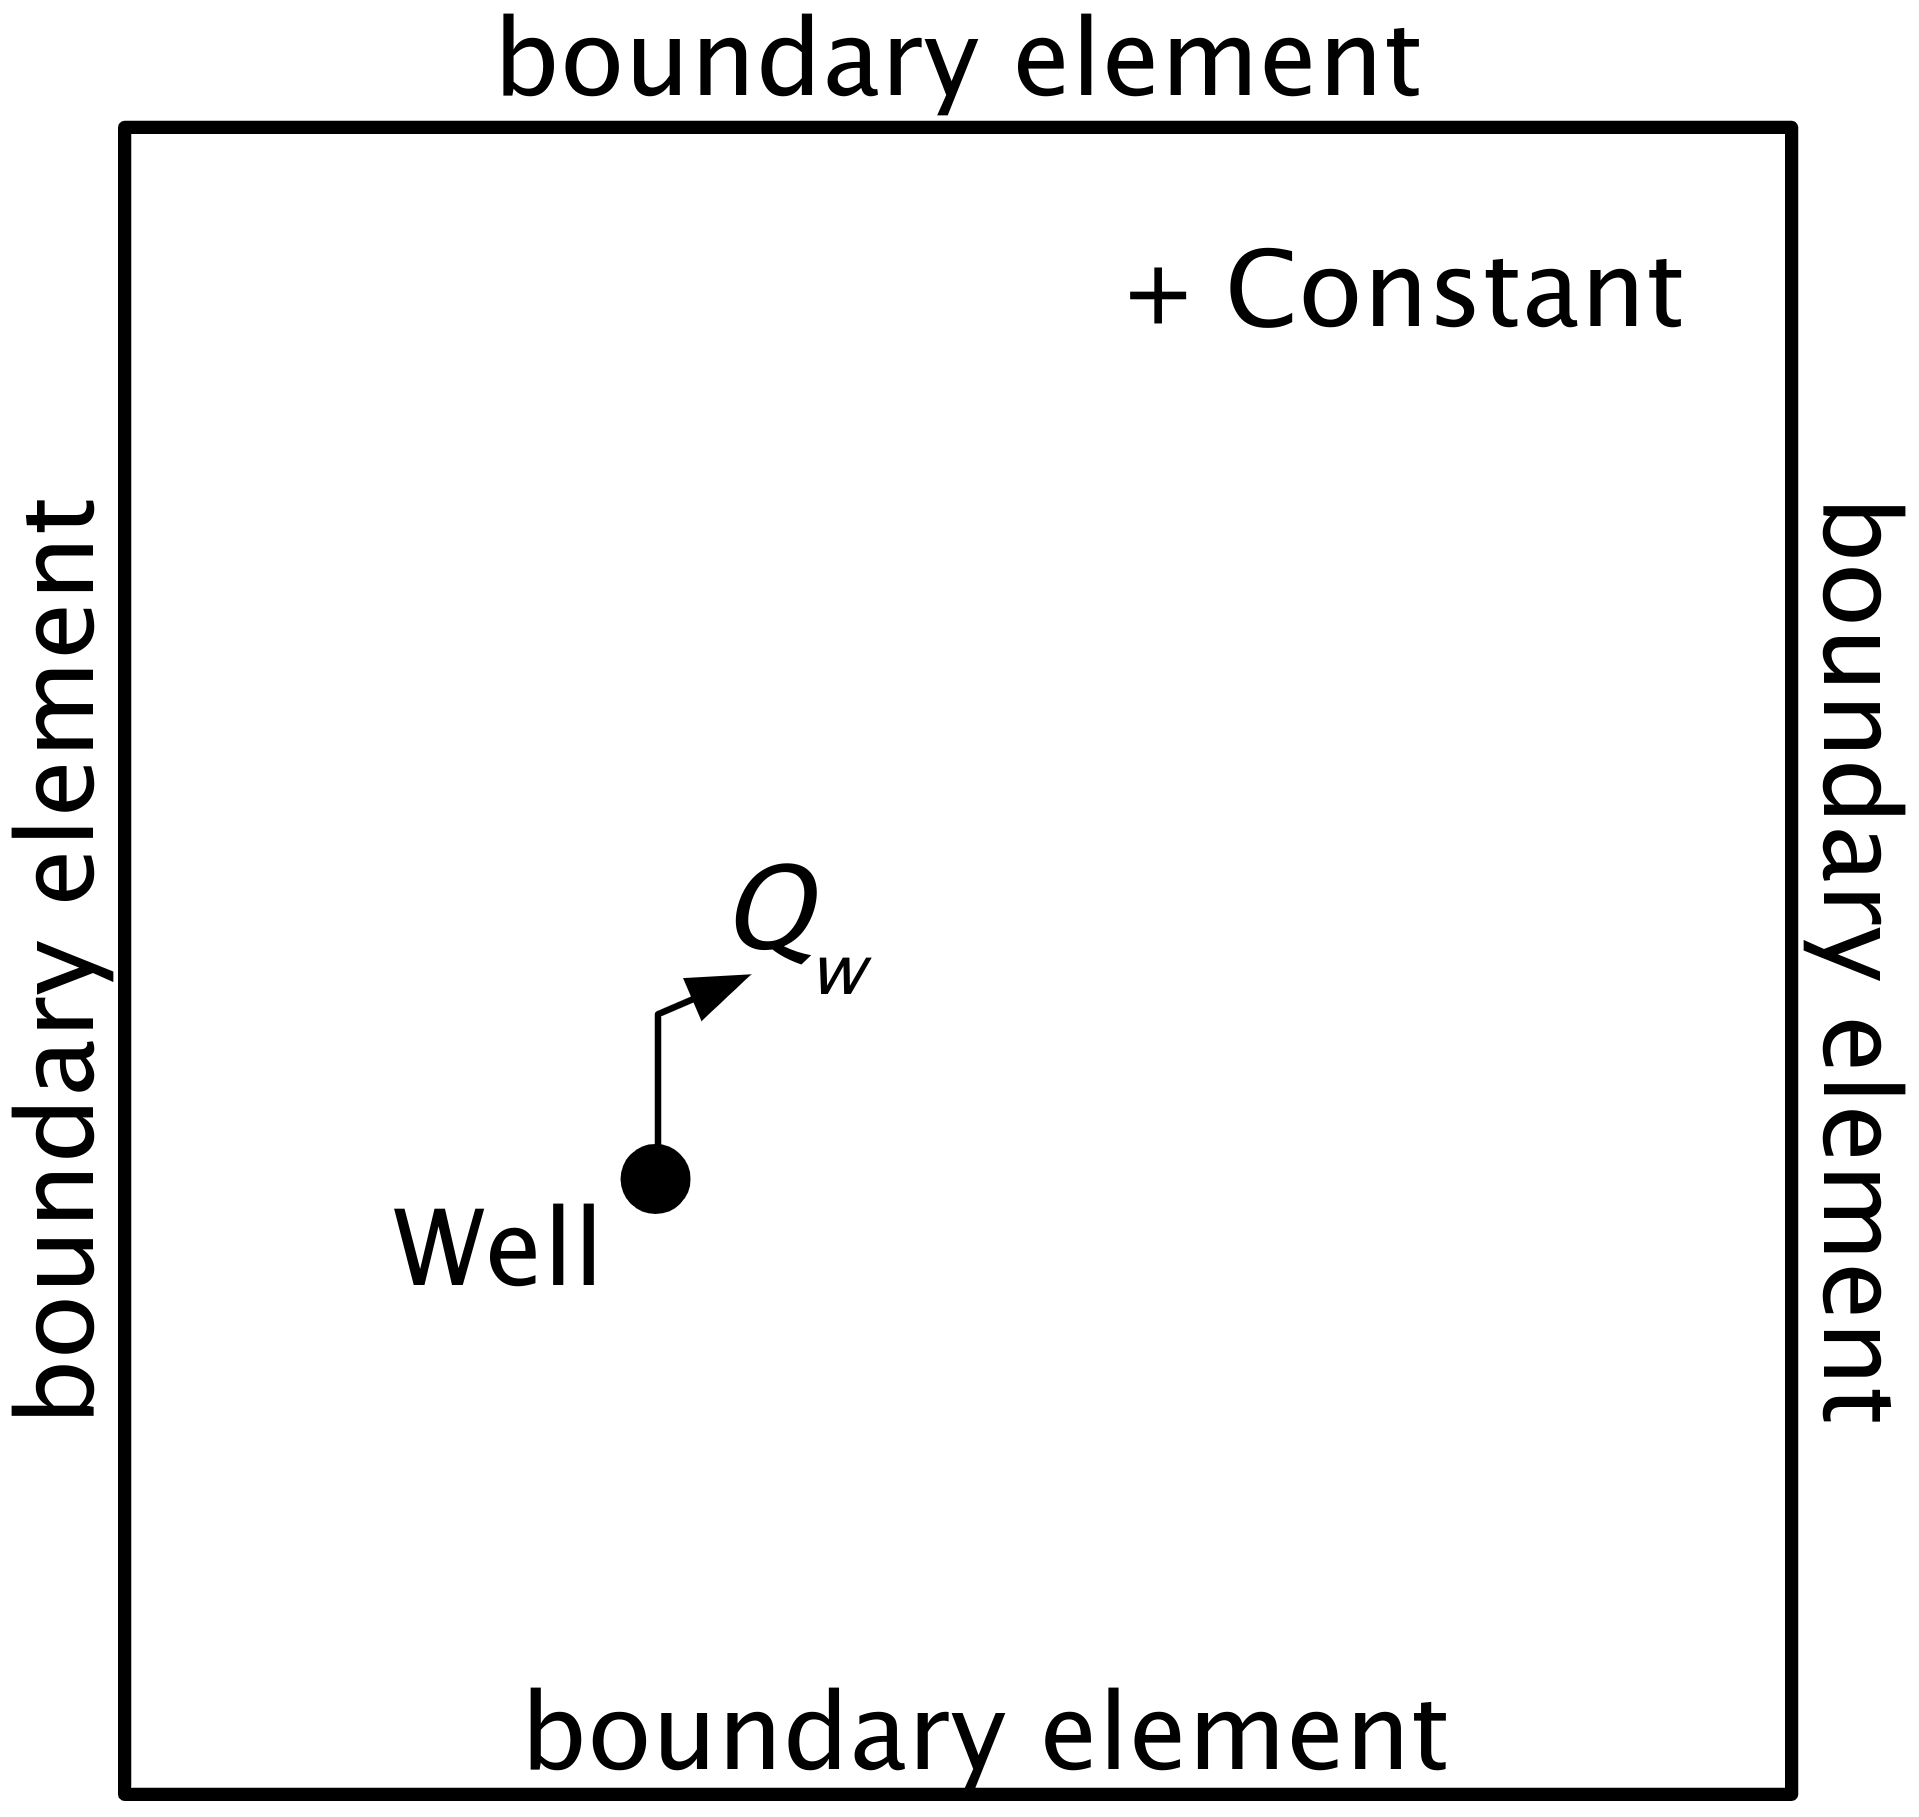
\includegraphics[height=100mm]{figures/AEM_of_FD_cell.png}
        \end{tikzfigure}
    
        \end{multicols}
    
    }

    \column{0.25}
    \block[bodyoffsety=5mm,titleoffsety=5mm,bodyverticalshift=-5mm]{Analytic Element Models}{

        \begin{tikzfigure}[An example of an Analytic Element Model.\par]
            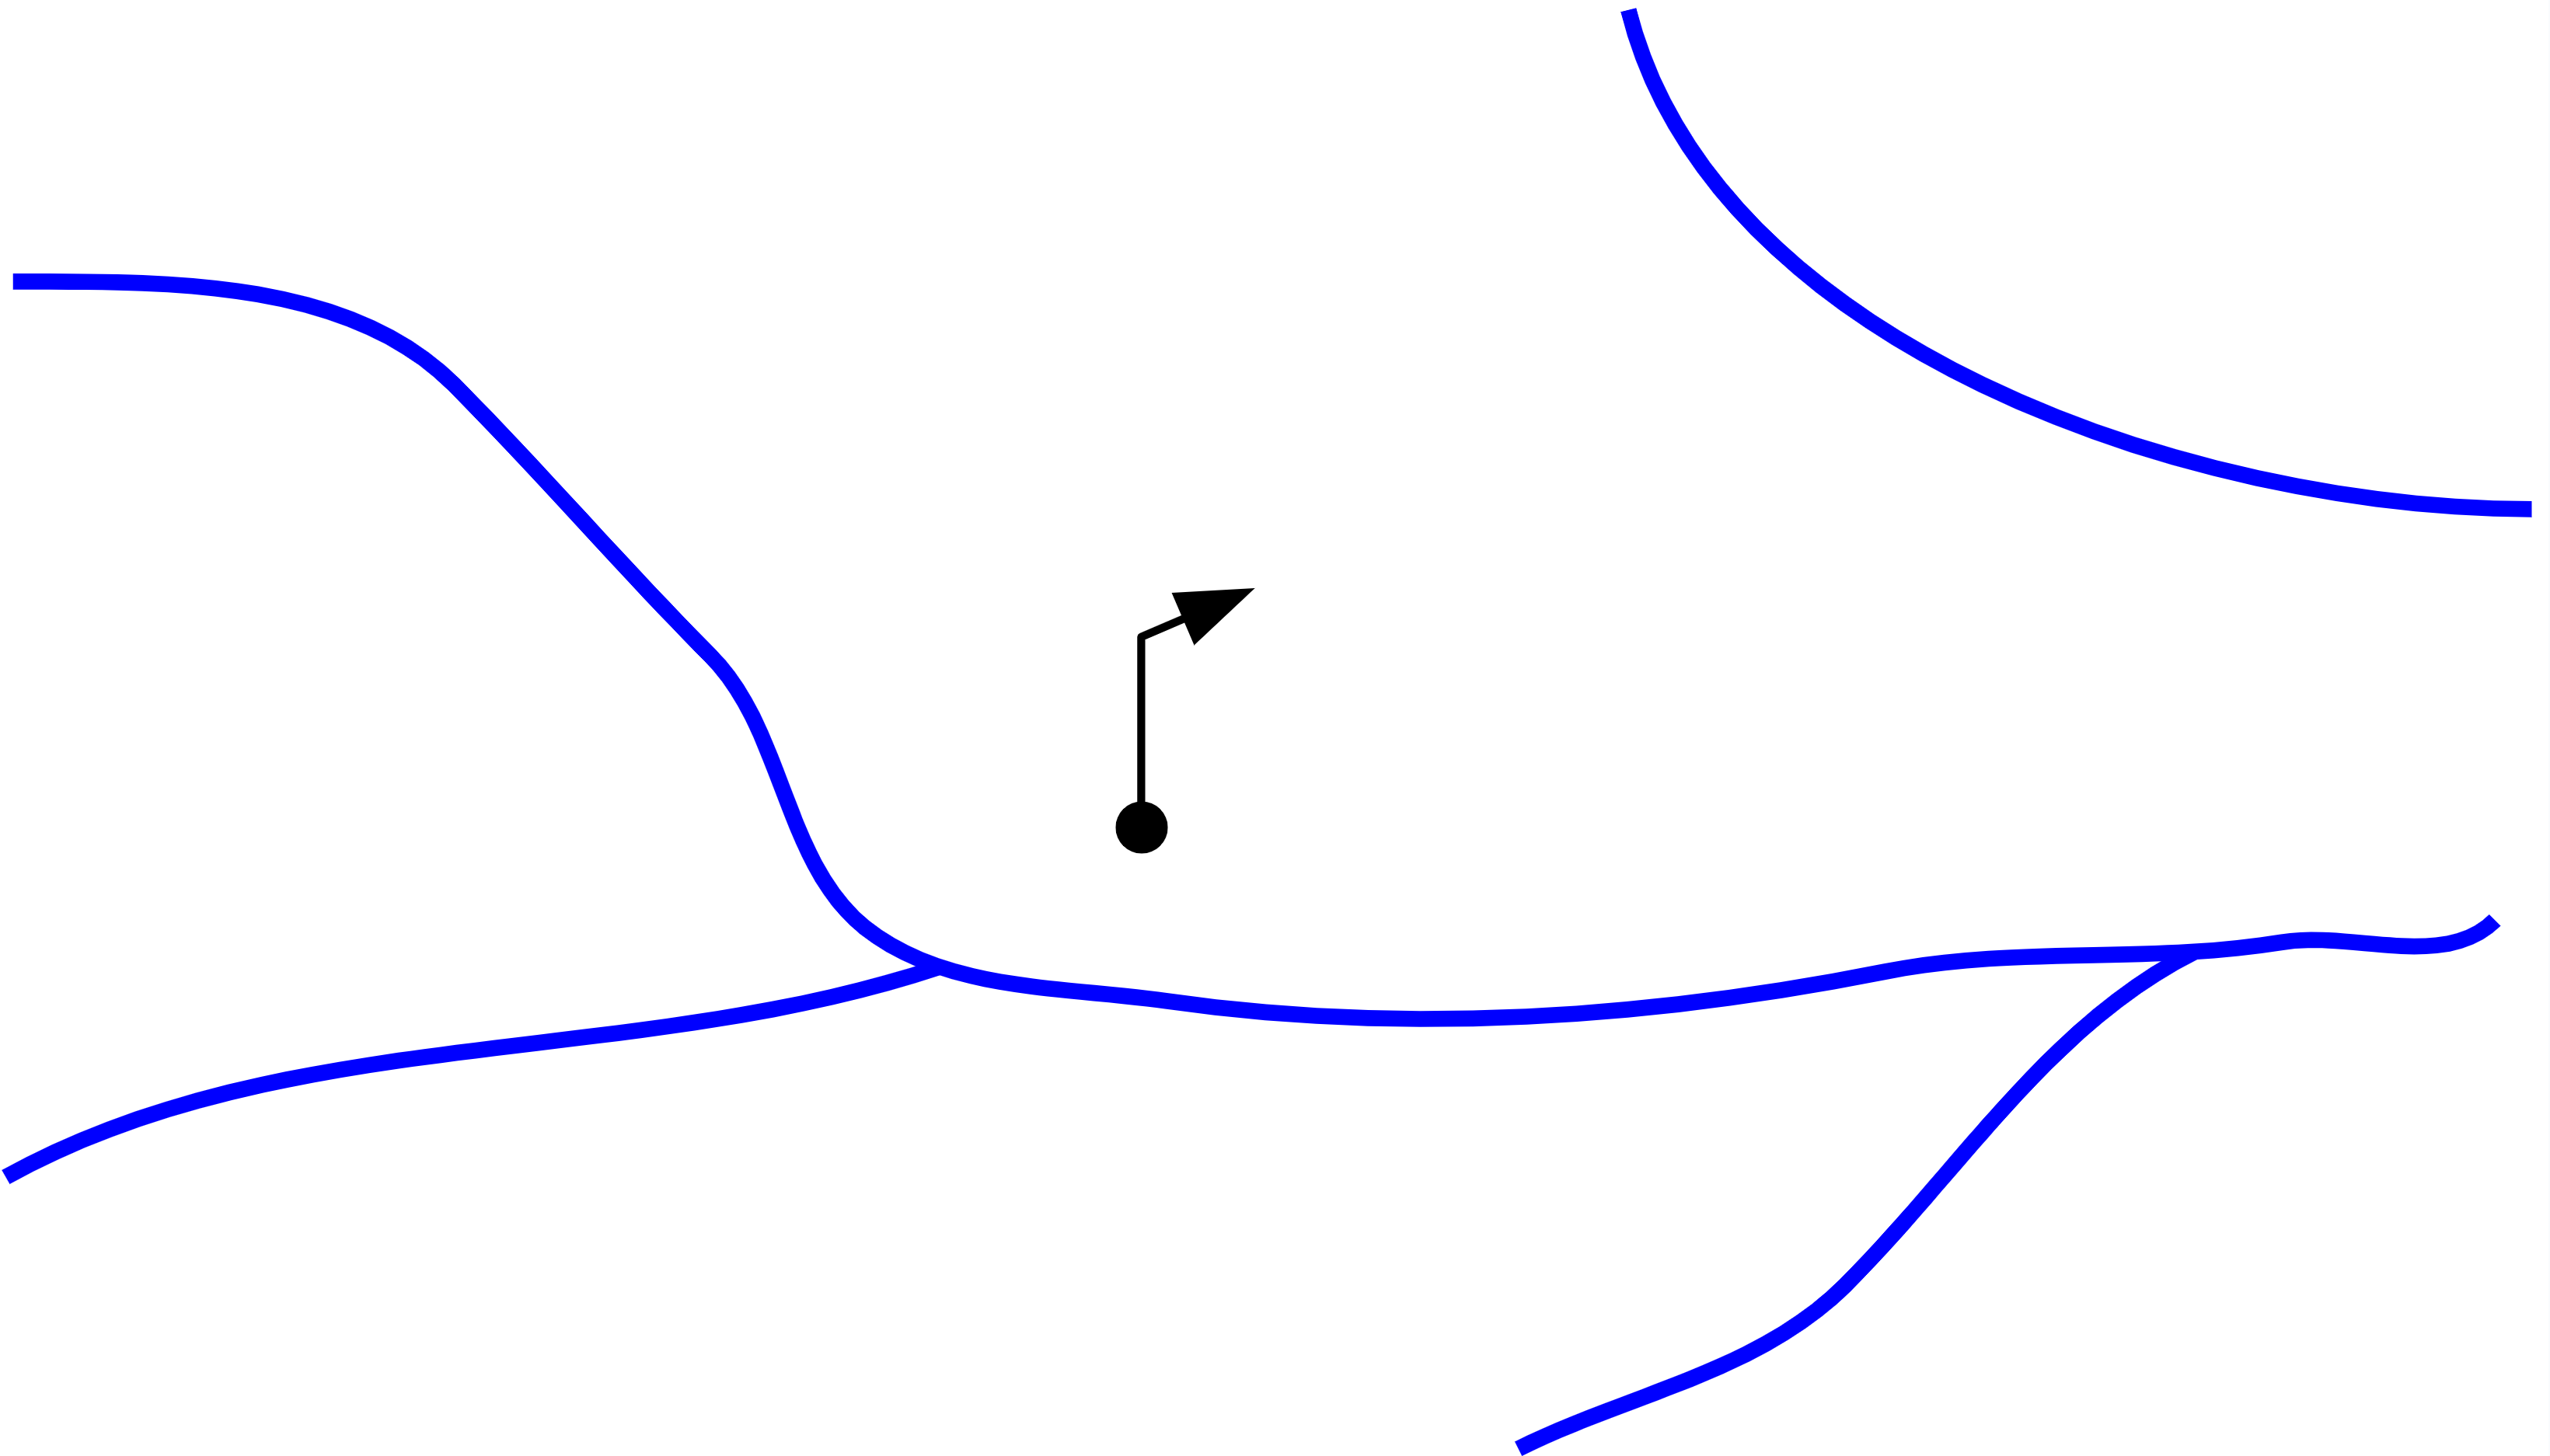
\includegraphics[width=\linewidth]{figures/AEM_example.png}
        \end{tikzfigure}

        \vspace{3mm}
        
        Advantages:
        \begin{itemize}[noitemsep]
            \item No grid! Head/flow at any point no spatial or temporal discretization required.
            \item Features can be modeled at exact locations, no snapping to grid.
        \end{itemize}
        
        \vspace{3mm}
        
        Disadvantages:
        \begin{itemize}[noitemsep]
            \item Modeling highly heterogeneous systems requires a lot of elements and is computationally intensive.
        \end{itemize}   

        \vspace{3mm}
        
        Implementation:
        \begin{itemize}[noitemsep]
            \item The analytic solutions used in the research were programmed in Python following the TimML object-oriented structure \citep{bakker_writing_2009,mark_bakker_analytical_2022}. Many more elements were added as part of researching the most flexible and robust method for coupling with FD models.
        \end{itemize}
}

    \column{0.25}
    \block[bodyoffsety=5mm,titleoffsety=5mm,bodyverticalshift=-5mm]{Finite Difference Models}{

        \begin{tikzfigure}[An example of a Finite Difference Model \citep{hughes_flopy_2023}.\par]
            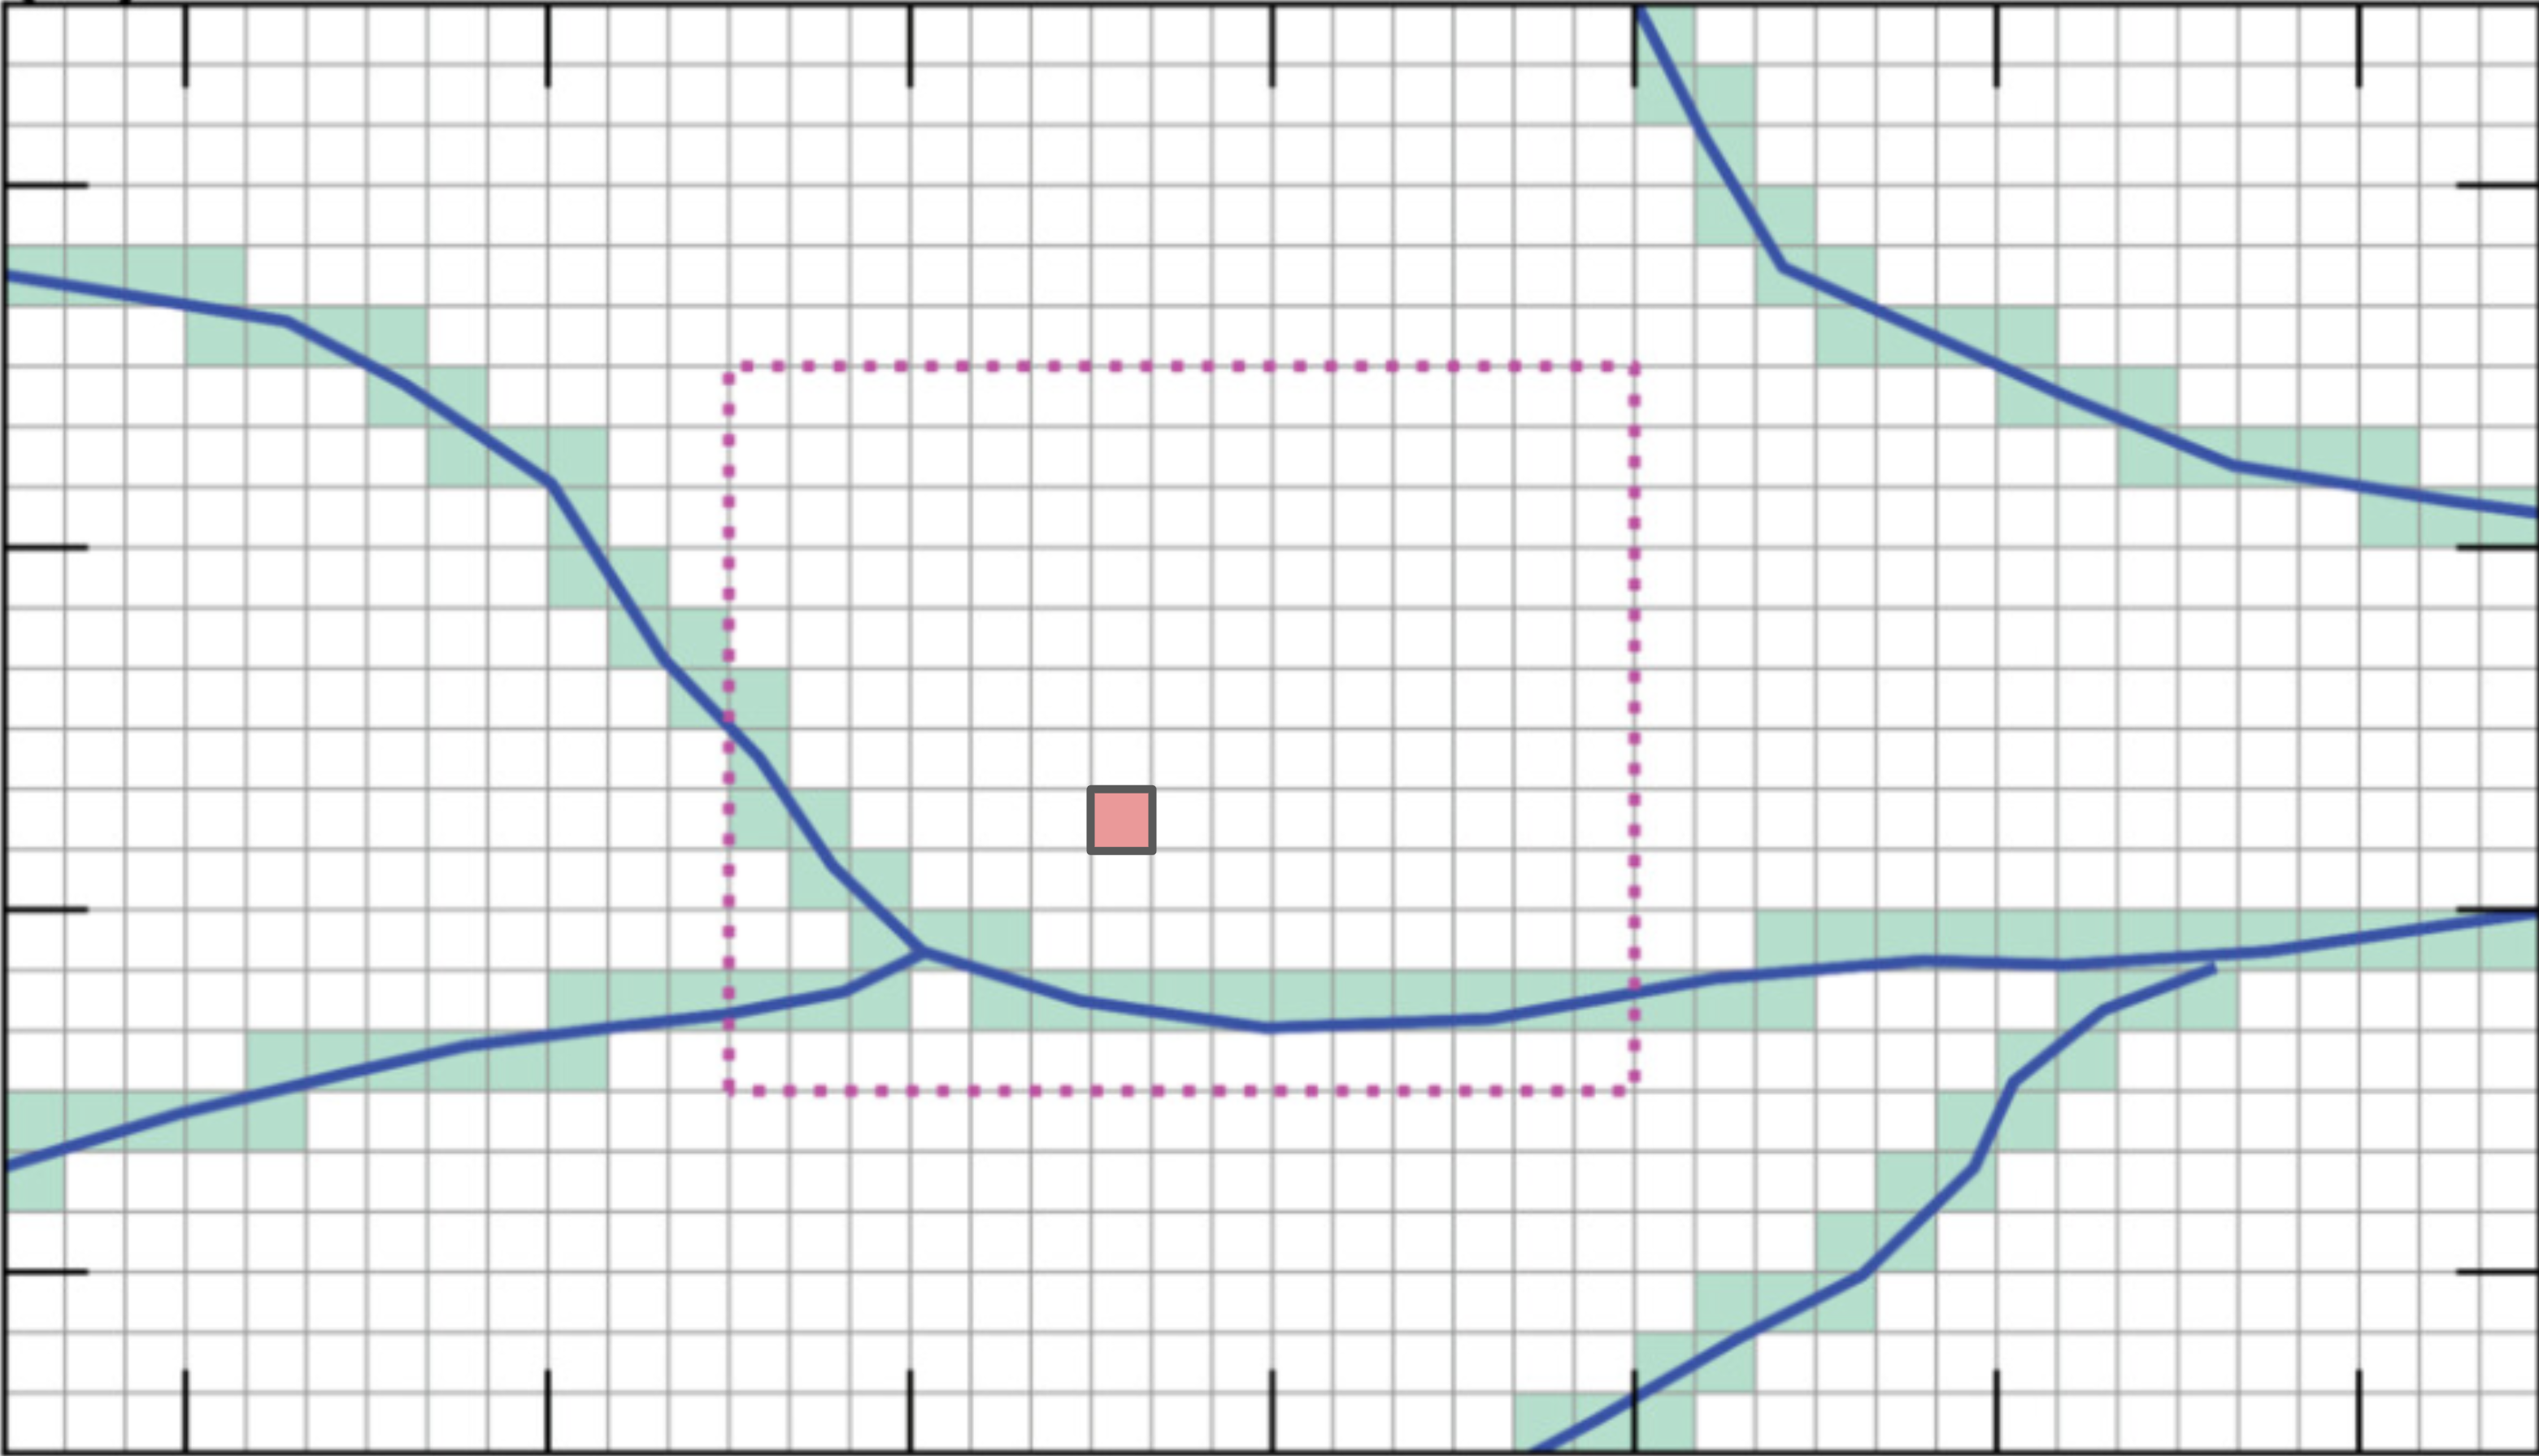
\includegraphics[width=\linewidth]{figures/FD_example.png}
        \end{tikzfigure}

        \vspace{3mm}
        
        Advantages:
        \begin{itemize}[noitemsep]
            \item Fast and efficient for large-scale heterogeneous problems.
            \item Large-scale regional models are often available as finite difference groundwater models.
        \end{itemize}

        \vspace{3mm}
        
        Disadvantages:
        \begin{itemize}[noitemsep]
            \item Spatial and temporal discretization have to be defined.
            \item Grid has to be adapted to local features.
        \end{itemize}   

        \vspace{3mm}
        
        Implementation:
        \begin{itemize}[noitemsep]
            \item A simple finite difference model for single confined aquifers was used in the research. The finite difference implementation was programmed in Python. Modflow 6 was not initially used as accessing and modifying the relevant parts of the code was inconvenient at this stage of the  project. 
        \end{itemize}   

        \vfill
}

\end{columns}

\begin{columns}
    \column{0.5}
    \block[bodyverticalshift=-8mm]{General Head Boundary Line Element}{
        \begin{multicols}{2}
            
        The boundary elements facilitate the communication between the AEM model and the FD model. The boundary element is set up as general head boundary. The normal flux $q_n$ over the element is uniform but unknown. The flux is driven by the difference between some specified head $h_\text{FD}$ and the mean head along the element $h_m$, multiplied by a conductance term $C$. The conductance is computed from the FD cell midpoint to the cell boundary. 

        \begin{equation}\label{eqn:ghb}
            Q_n = q_n \Delta y \Delta z = C \left( h_\text{FD} - h_m \right) 
        \end{equation}

        \vspace{3mm}
        
        The analytic solution of the boundary element is derived through separation of variables in elliptic coordinates \citep{bakker_derivation_2008}. The solutions for line-sinks and line-doublets are added together as this gave the most accurate results. 
        
        \begin{tikzfigure}[Schematic showing the general head boundary element between a FD cell and an AEM model.\par]
            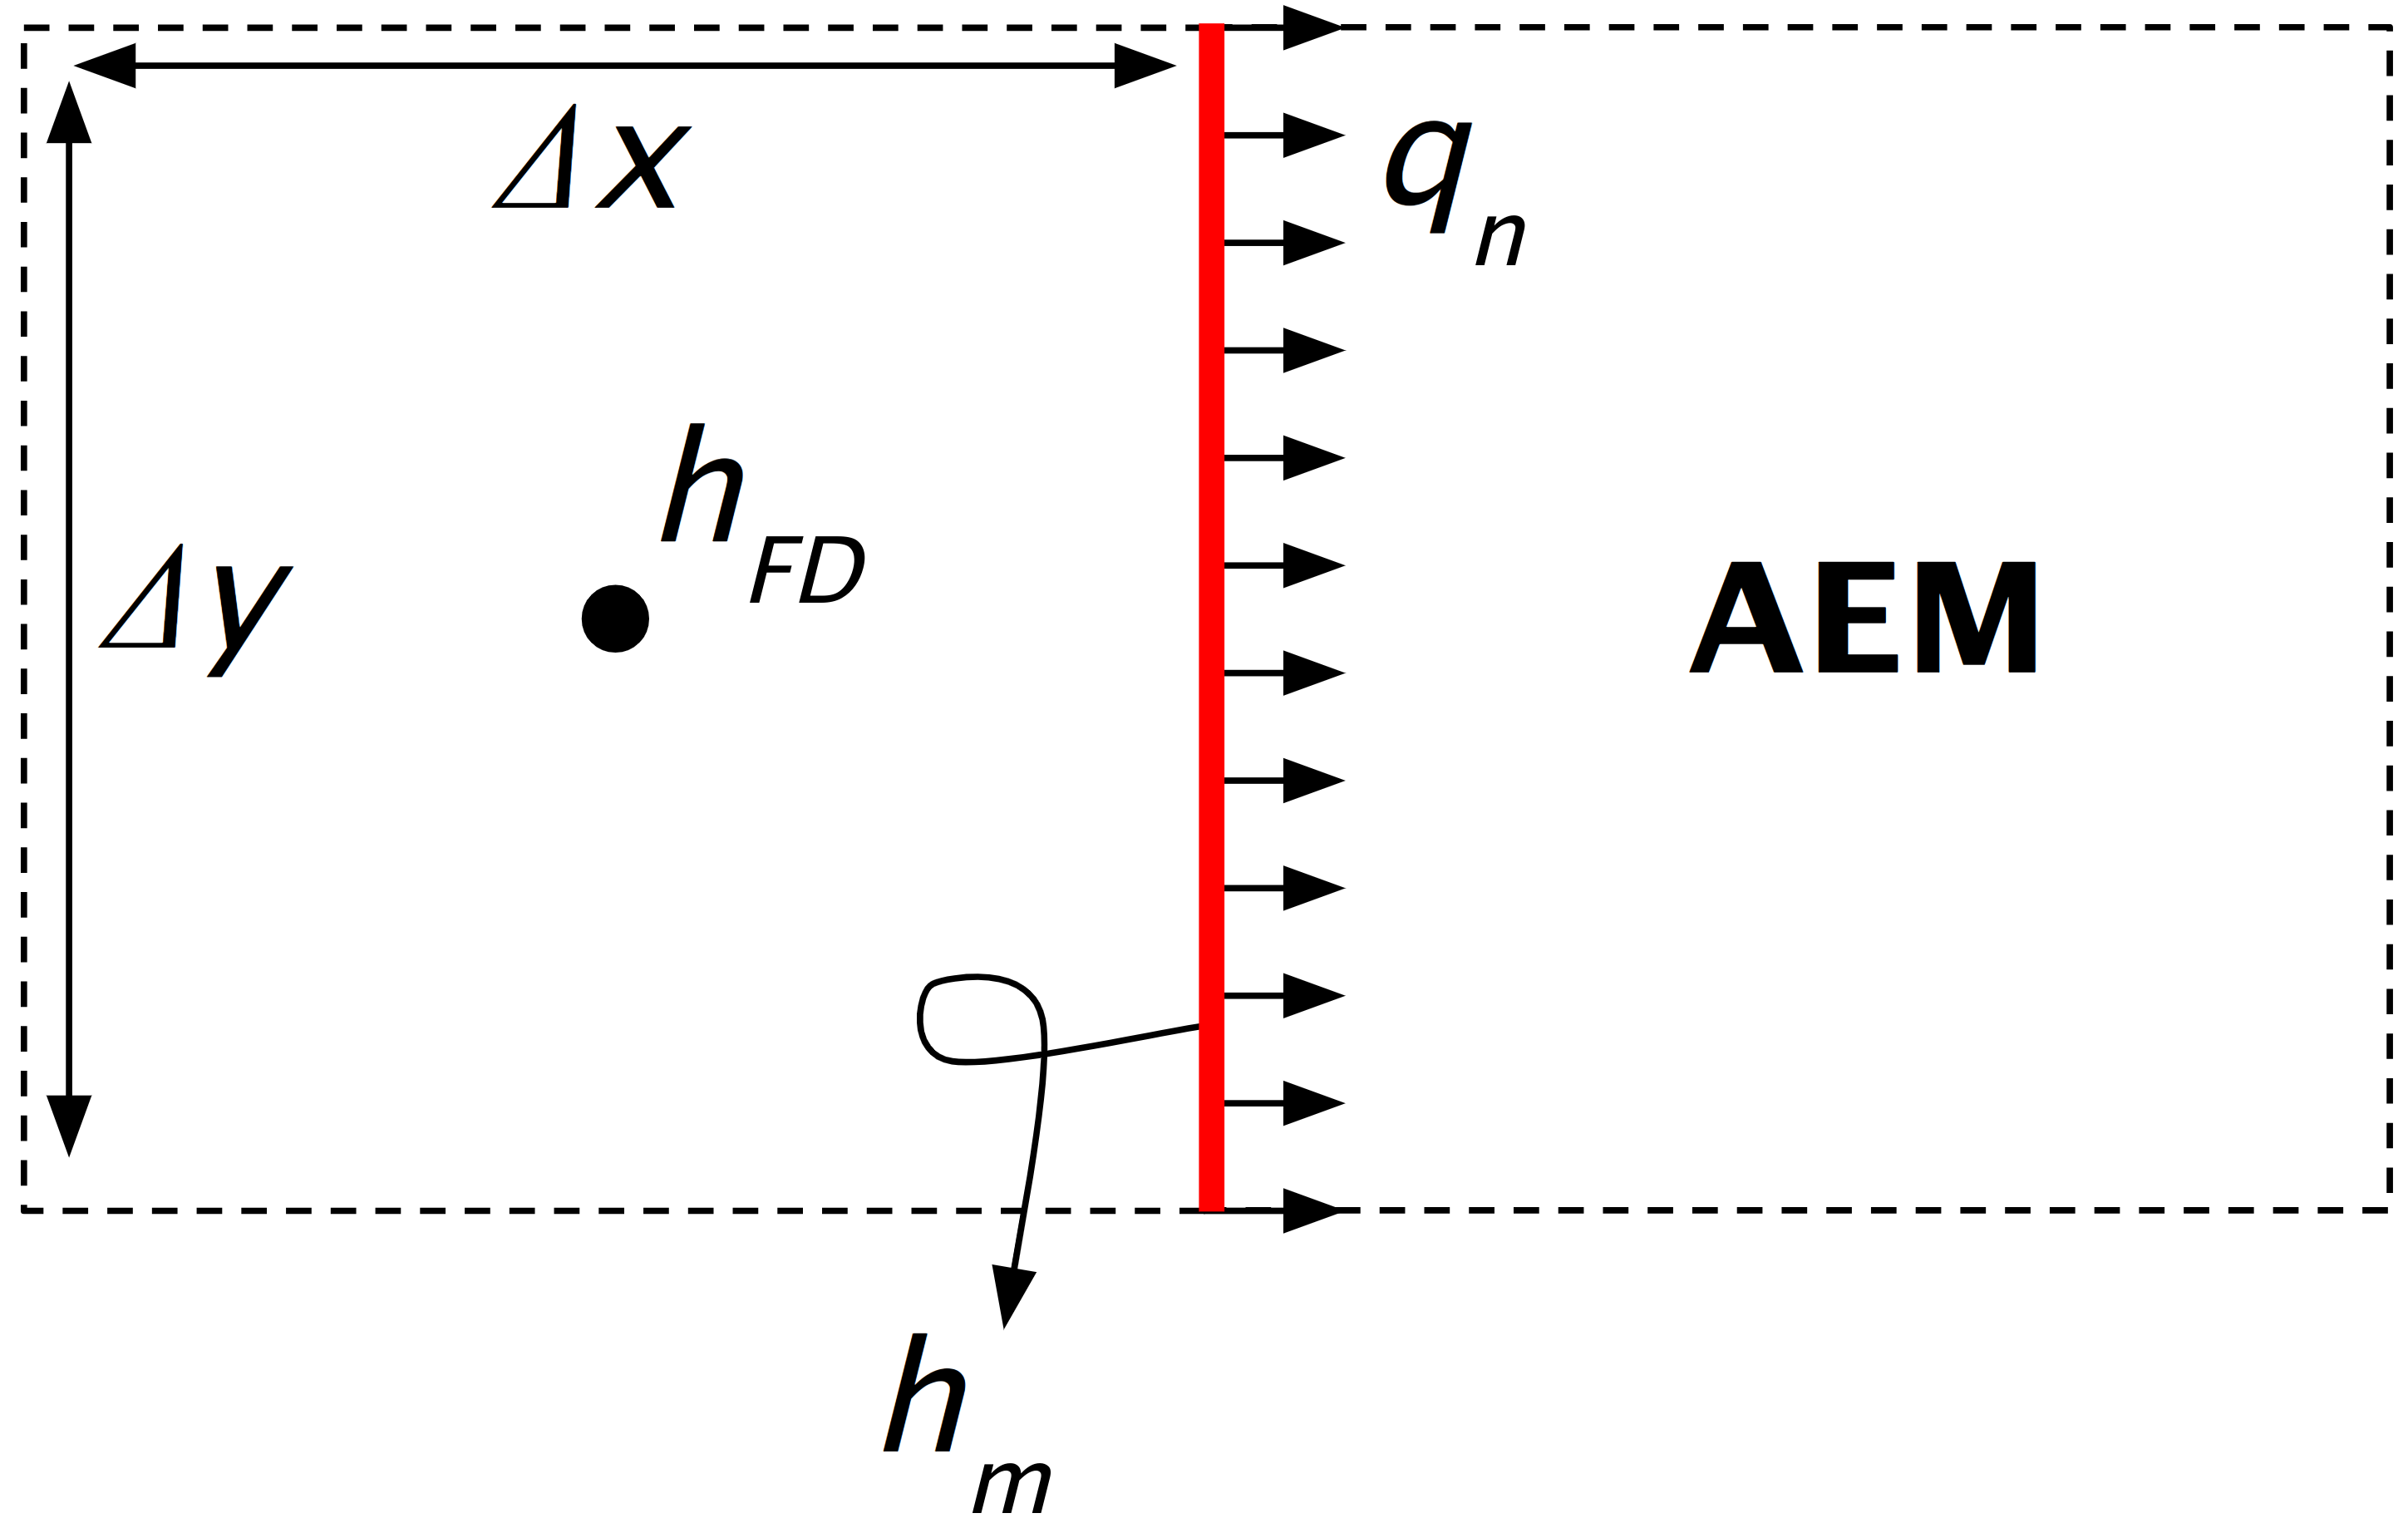
\includegraphics[height=80mm]{figures/boundary_element.png}
        \end{tikzfigure}
        
        \end{multicols}
    }
    
    \column{0.5}
    \block[bodyverticalshift=-8mm]{Solving AEM and FD simultaneously}{

    \begin{multicols}{2}
        The equations for the FD model and AEM model are written in matrix form $\mathbf{A}\vec{x} = b$.    
        The FD equation for replaced cell is removed. The equations for the neighboring FD cells are modified:
        
        
        \begin{itemize}[noitemsep]
            \item the mean head along the boundary elements is substituted into the FD equations
            \item The conductances are adjusted accordingly, from cell midpoint to cell boundary 
        \end{itemize} 
        
        The AEM equations use the head from the neighboring FD cells to compute the the flux entering the AEM model (Eq. \ref{eqn:ghb}). 

        \vspace{3mm}
        Solving for $\vec{x}$ yields the heads of the FD cells and the parameters of the analytic elements.
        
        \begin{tikzfigure}[The coefficients of the equations (matrix $\mathbf{A}$) for the coupled FD+AEM solution.\par]
            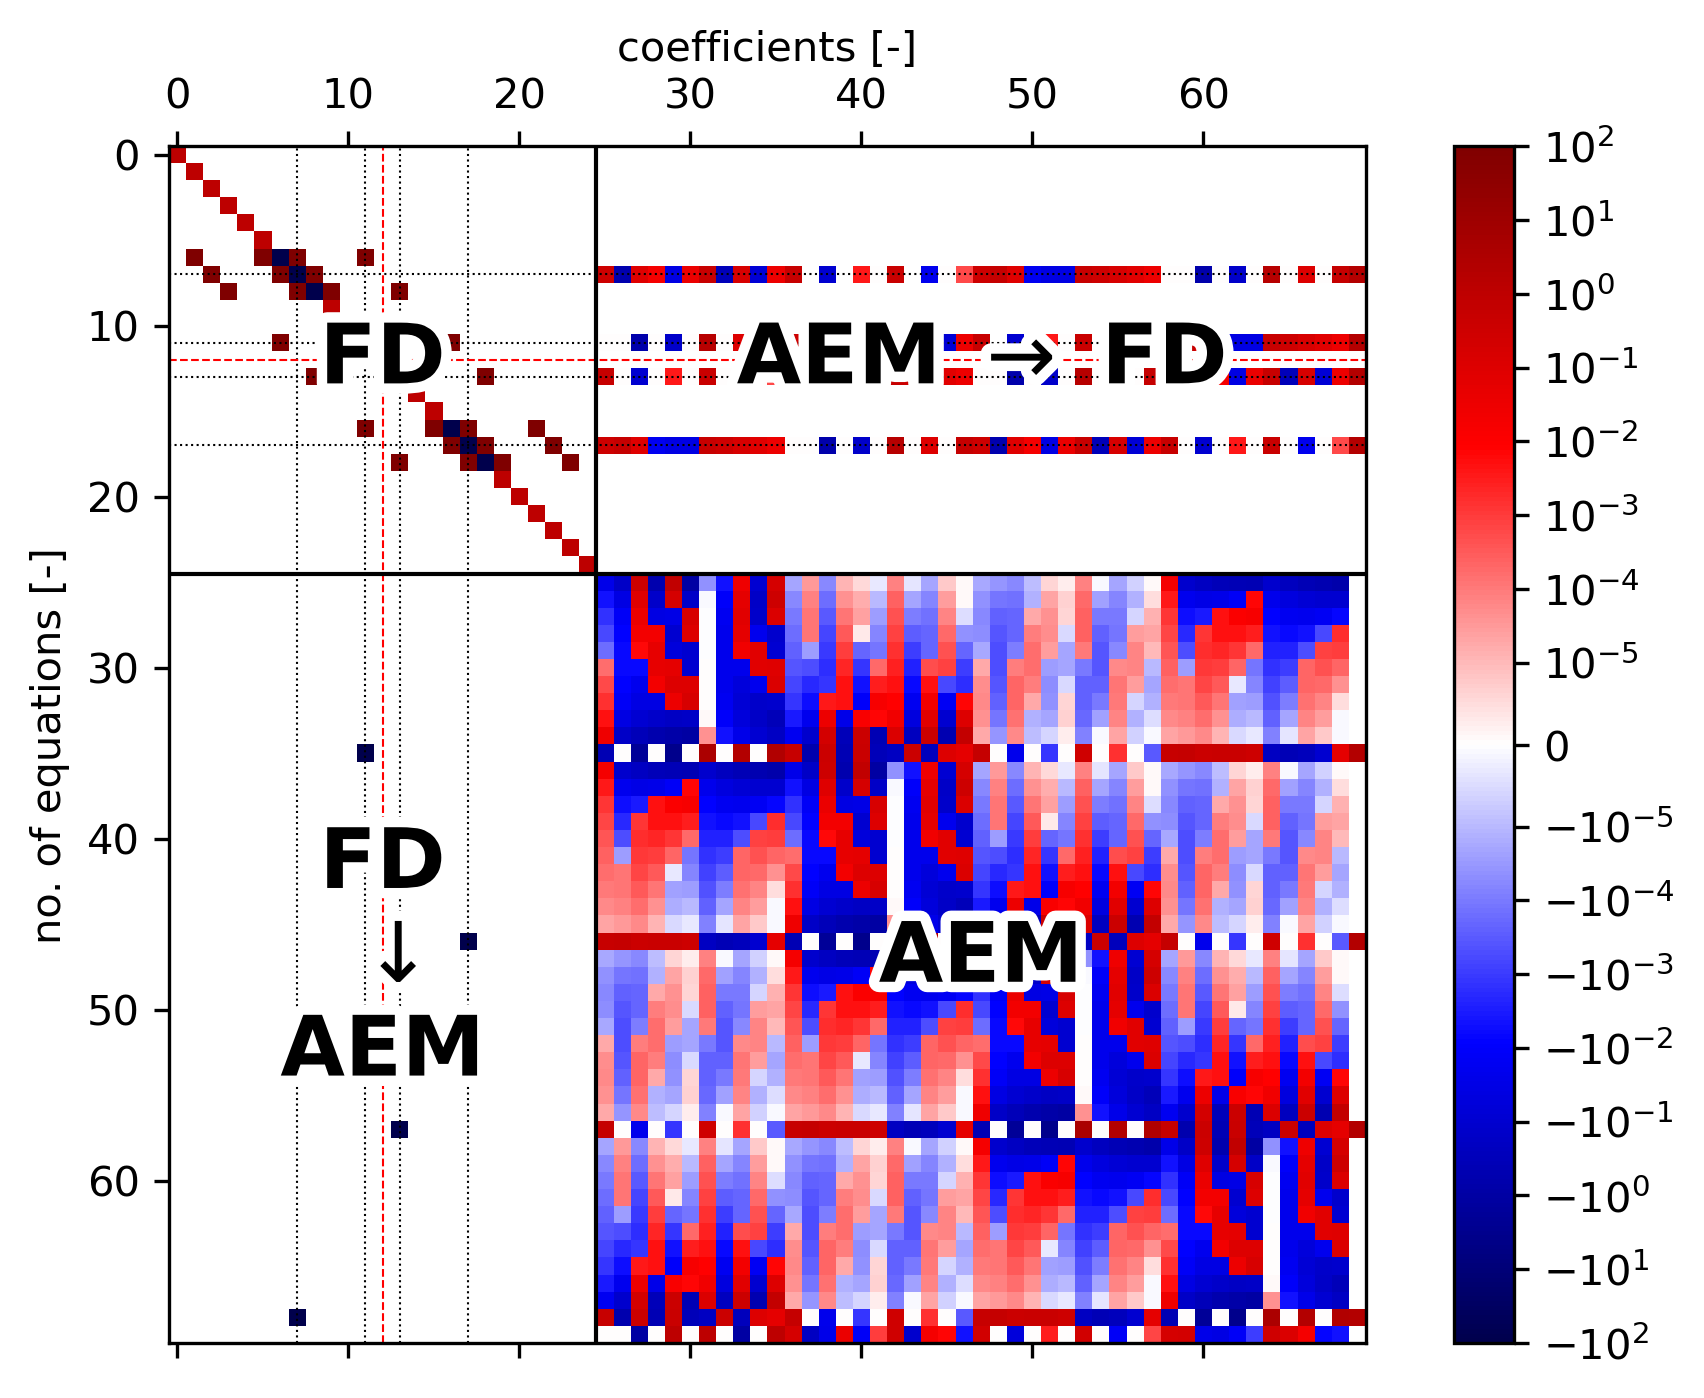
\includegraphics[height=120mm]{figures/mat_fd+aem.png}
        \end{tikzfigure}
    \end{multicols}
    
    }

\end{columns}
\begin{columns}

    \column{0.5}
    \block[bodyverticalshift=-8mm]{Benchmark Problem 1: Two Wells in Uniform Flow}{
        
        \begin{multicols}{3}
        
            Two wells are pumping from a confined aquifer with uniform flow from west to east. The eastern well is pumping at 75 m$^3$/d and the western well is pumping at 50 m$^3$/d. The FD model dimensions are 5$\times$5. 

            \begin{tikztable}[Model properties\par\label{tab:modelparams}]
                \centering
                \begin{tabular}{lrl}
                    \toprule
                    Parameter & Value & Units      \\
                    \midrule
                    Aquifer thickness & 10 & m \\
                    Horizontal conductivity & 10 & m/d \\
                    Porosity & 0.3 & - \\
                    Uniform flow & 0.001 & m/m \\
                    \bottomrule
                \end{tabular}
            \end{tikztable}

            \begin{tikzfigure}[Example model with 2 wells in uniform flow.\par]
                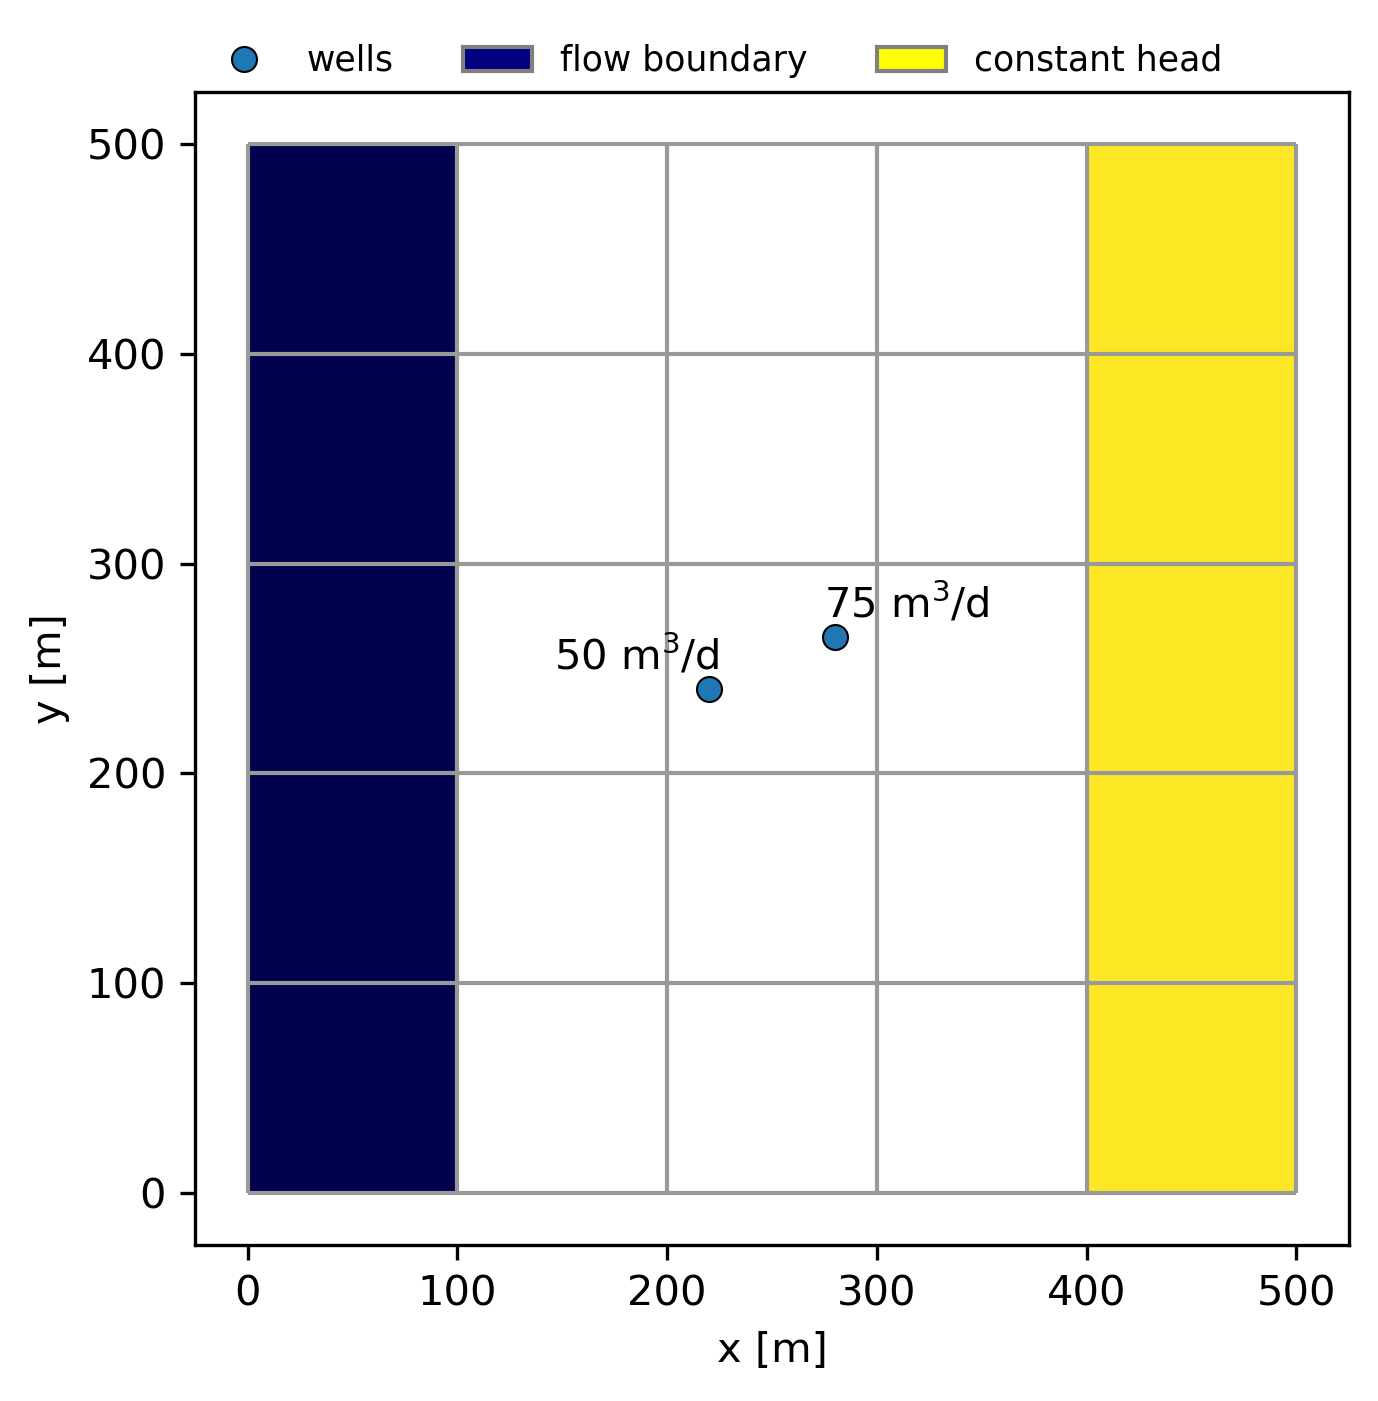
\includegraphics[width=0.75\linewidth]{figures/b04_fd_model_boundaries.png}
            \end{tikzfigure}

            The wells are both located within one cell in the FD model. The FD model is therefore not able to compute separate capture zones for each well. The coupled FD+AEM model is able to closely match the exact solution, despite the coarse 100 x 100 m resolution of the FD model.

        \end{multicols}

        \begin{tikzfigure}[Comparison of particle tracks for FD model, coupled FD and AEM model and the exact analytic solution.\par]
            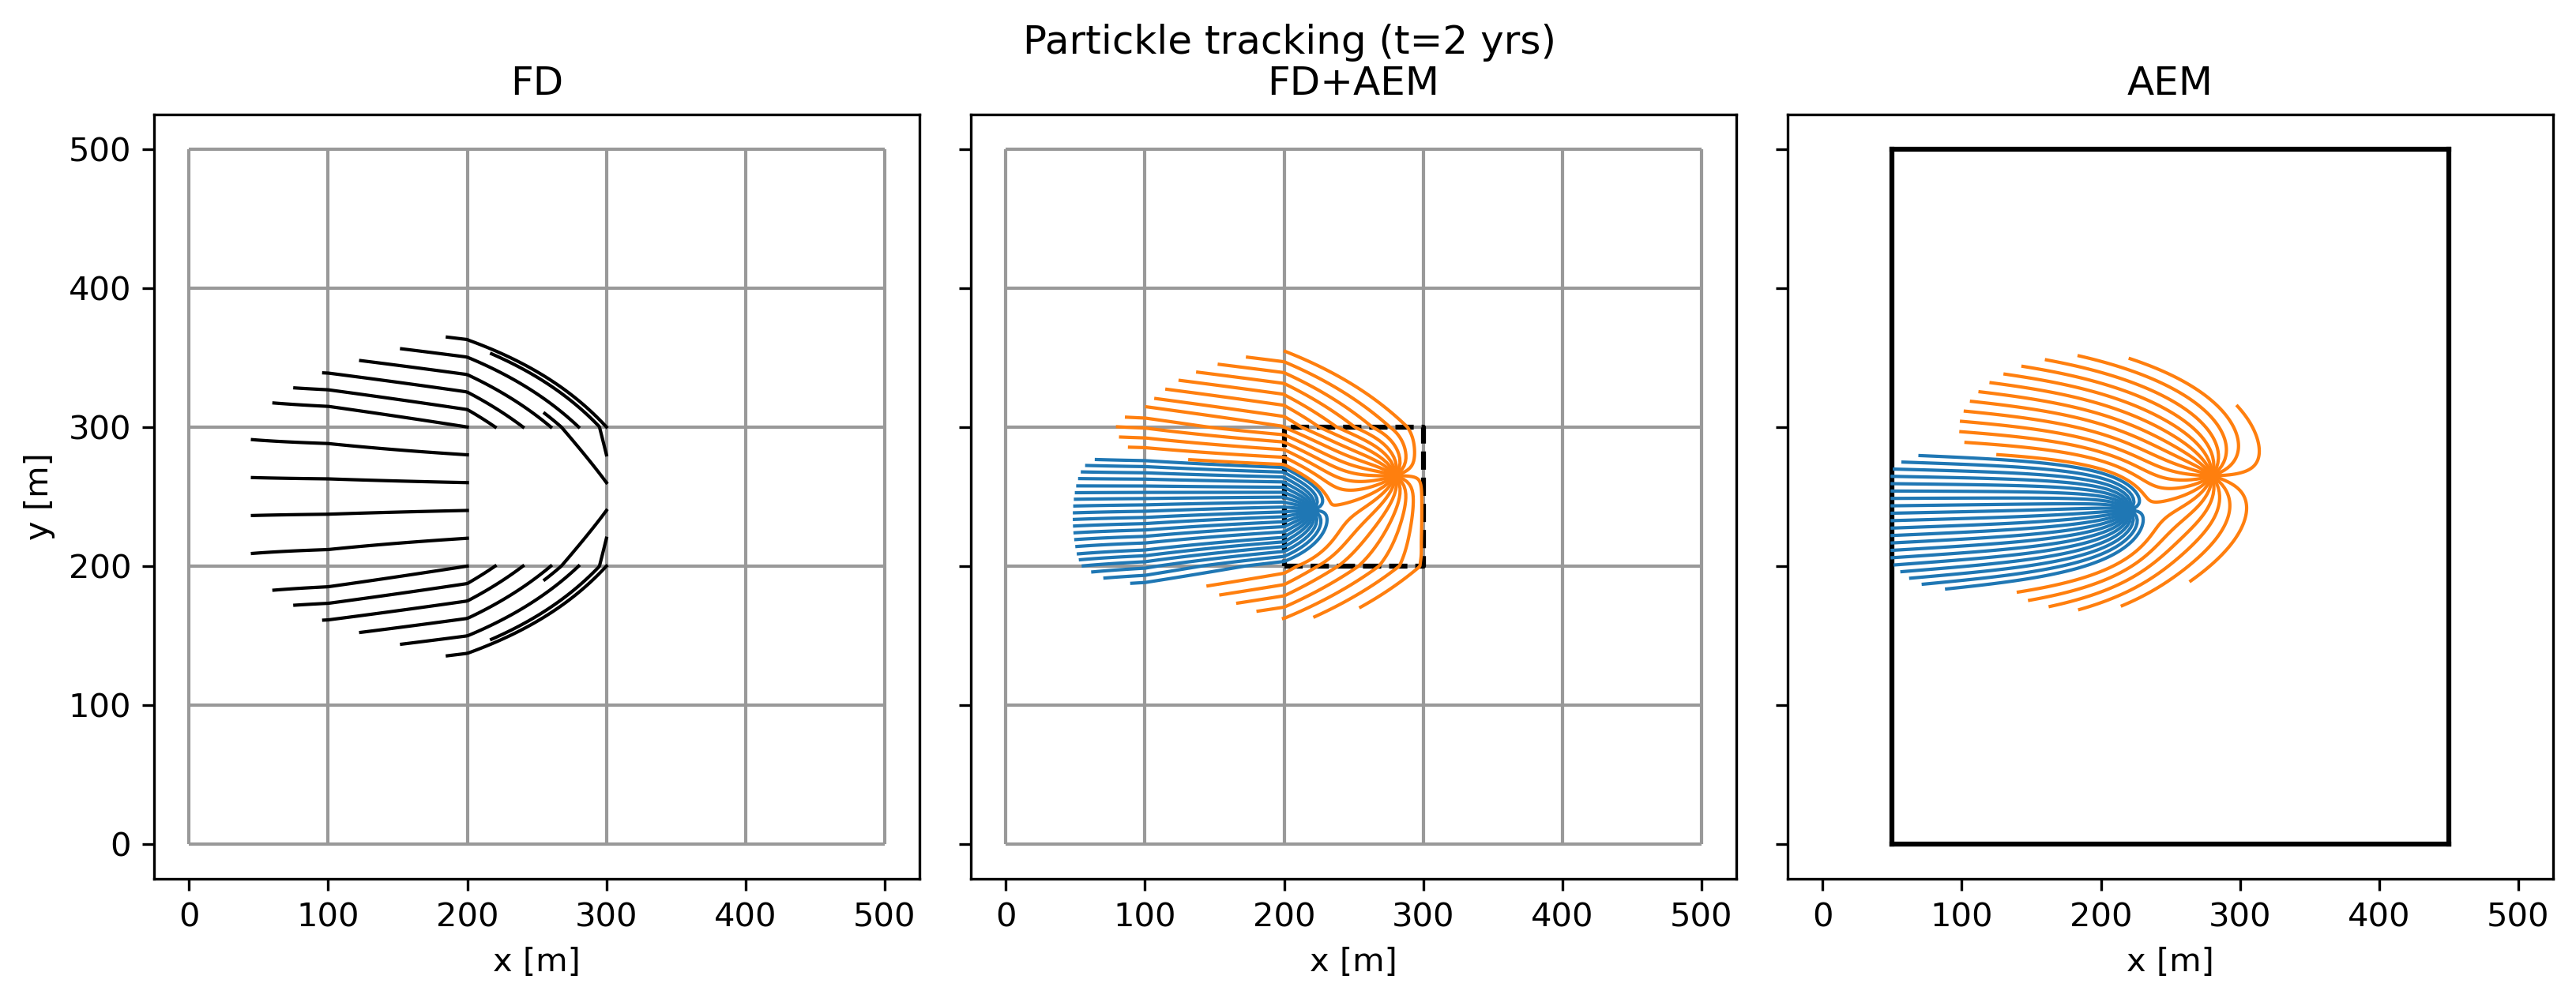
\includegraphics[width=\linewidth]{figures/b04_capture_zone.png}
        \end{tikzfigure}

    }

    \column{0.5}
    \block[bodyverticalshift=-8mm]{Benchmark Problem 2: Pumping and Injection in One Cell}{

        \begin{multicols}{3}

            An injection and a pumping well of equal magnitude supply and extract water in a confined aquifer at a rate of 150 m$^3$/d. Both wells lie within the same cell in the FD model. The model is bounded by a constant head boundary. The model parameters are shown in Table \ref{tab:modelparams}.

            The FD model cannot compute a sensible solution since the net pumping rate within the cell is 0 m$^3$/d. The coupled FD+AEM solution provides a reasonable estimate of the flow-net and the 15-year capture zone compared to the exact solution. 

            \begin{tikzfigure}[Example model with injection and pumping in one cell.\par]
                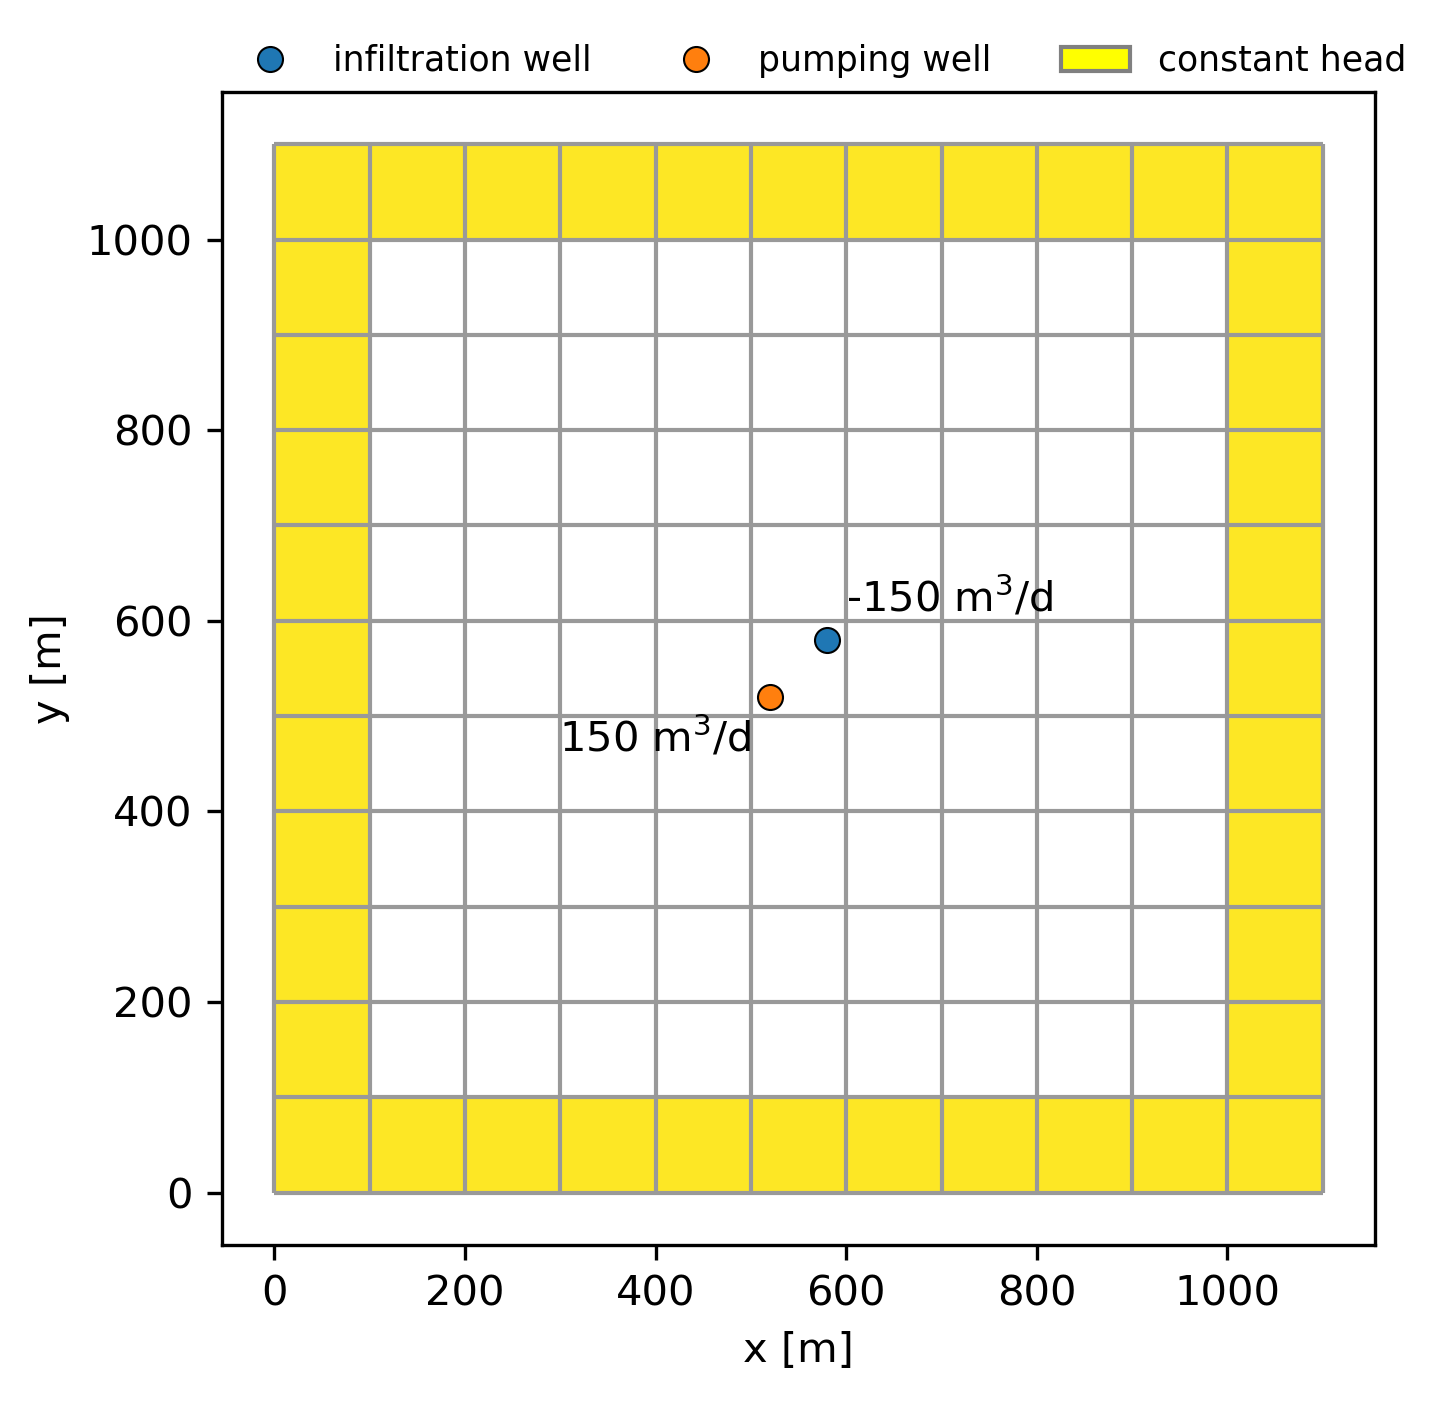
\includegraphics[width=0.75\linewidth]{figures/b05_fd_model_boundaries.png}
            \end{tikzfigure}

            \begin{tikzfigure}[Flow net of the coupled FD+AEM solution and the exact solution.\par]
                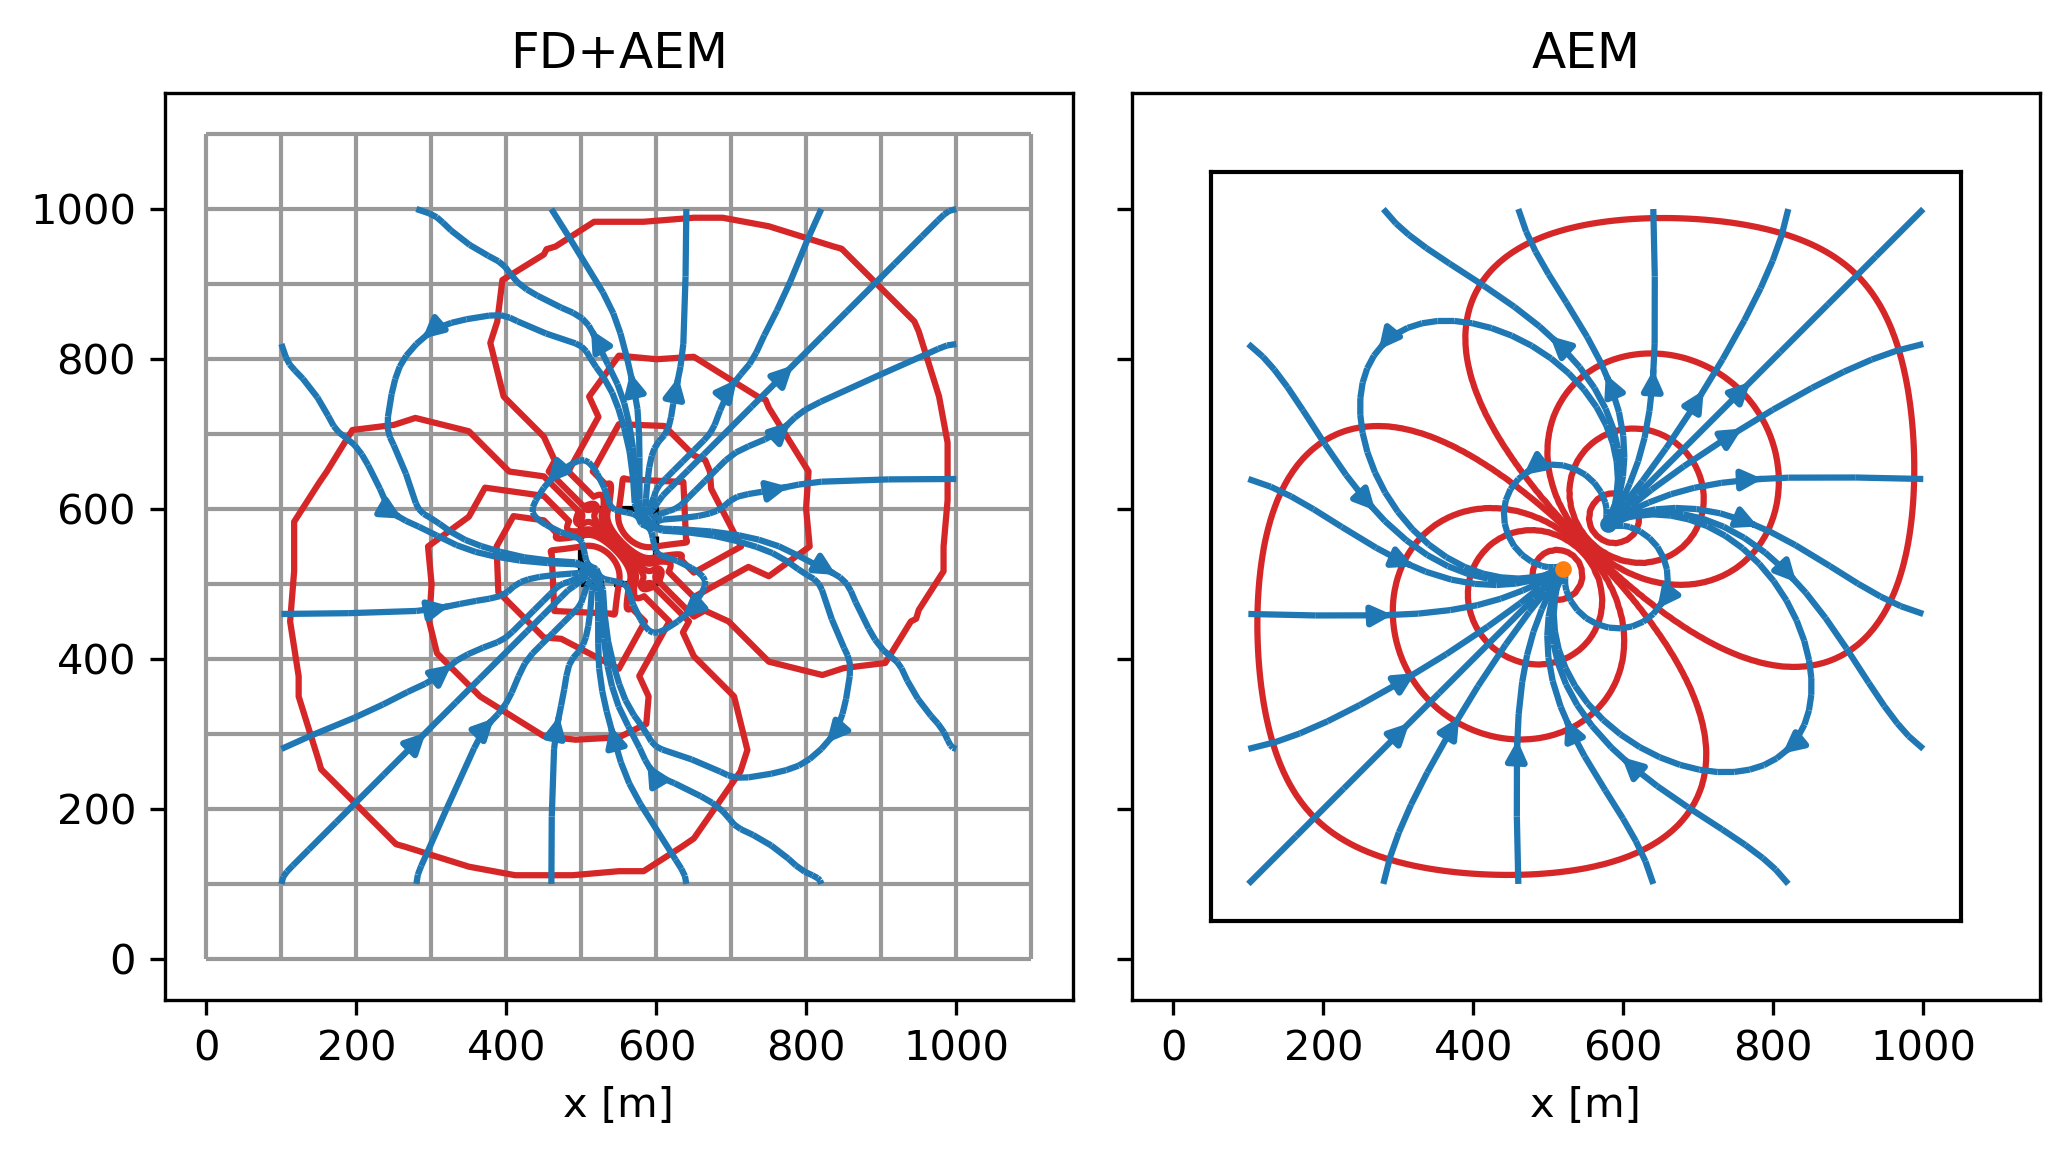
\includegraphics[width=\linewidth]{figures/b05_flow_net.png}
            \end{tikzfigure}
            
        \end{multicols}


        \begin{tikzfigure}[Comparison of particle tracks for FD model, coupled FD+AEM model and the exact analytic solution.\par]
            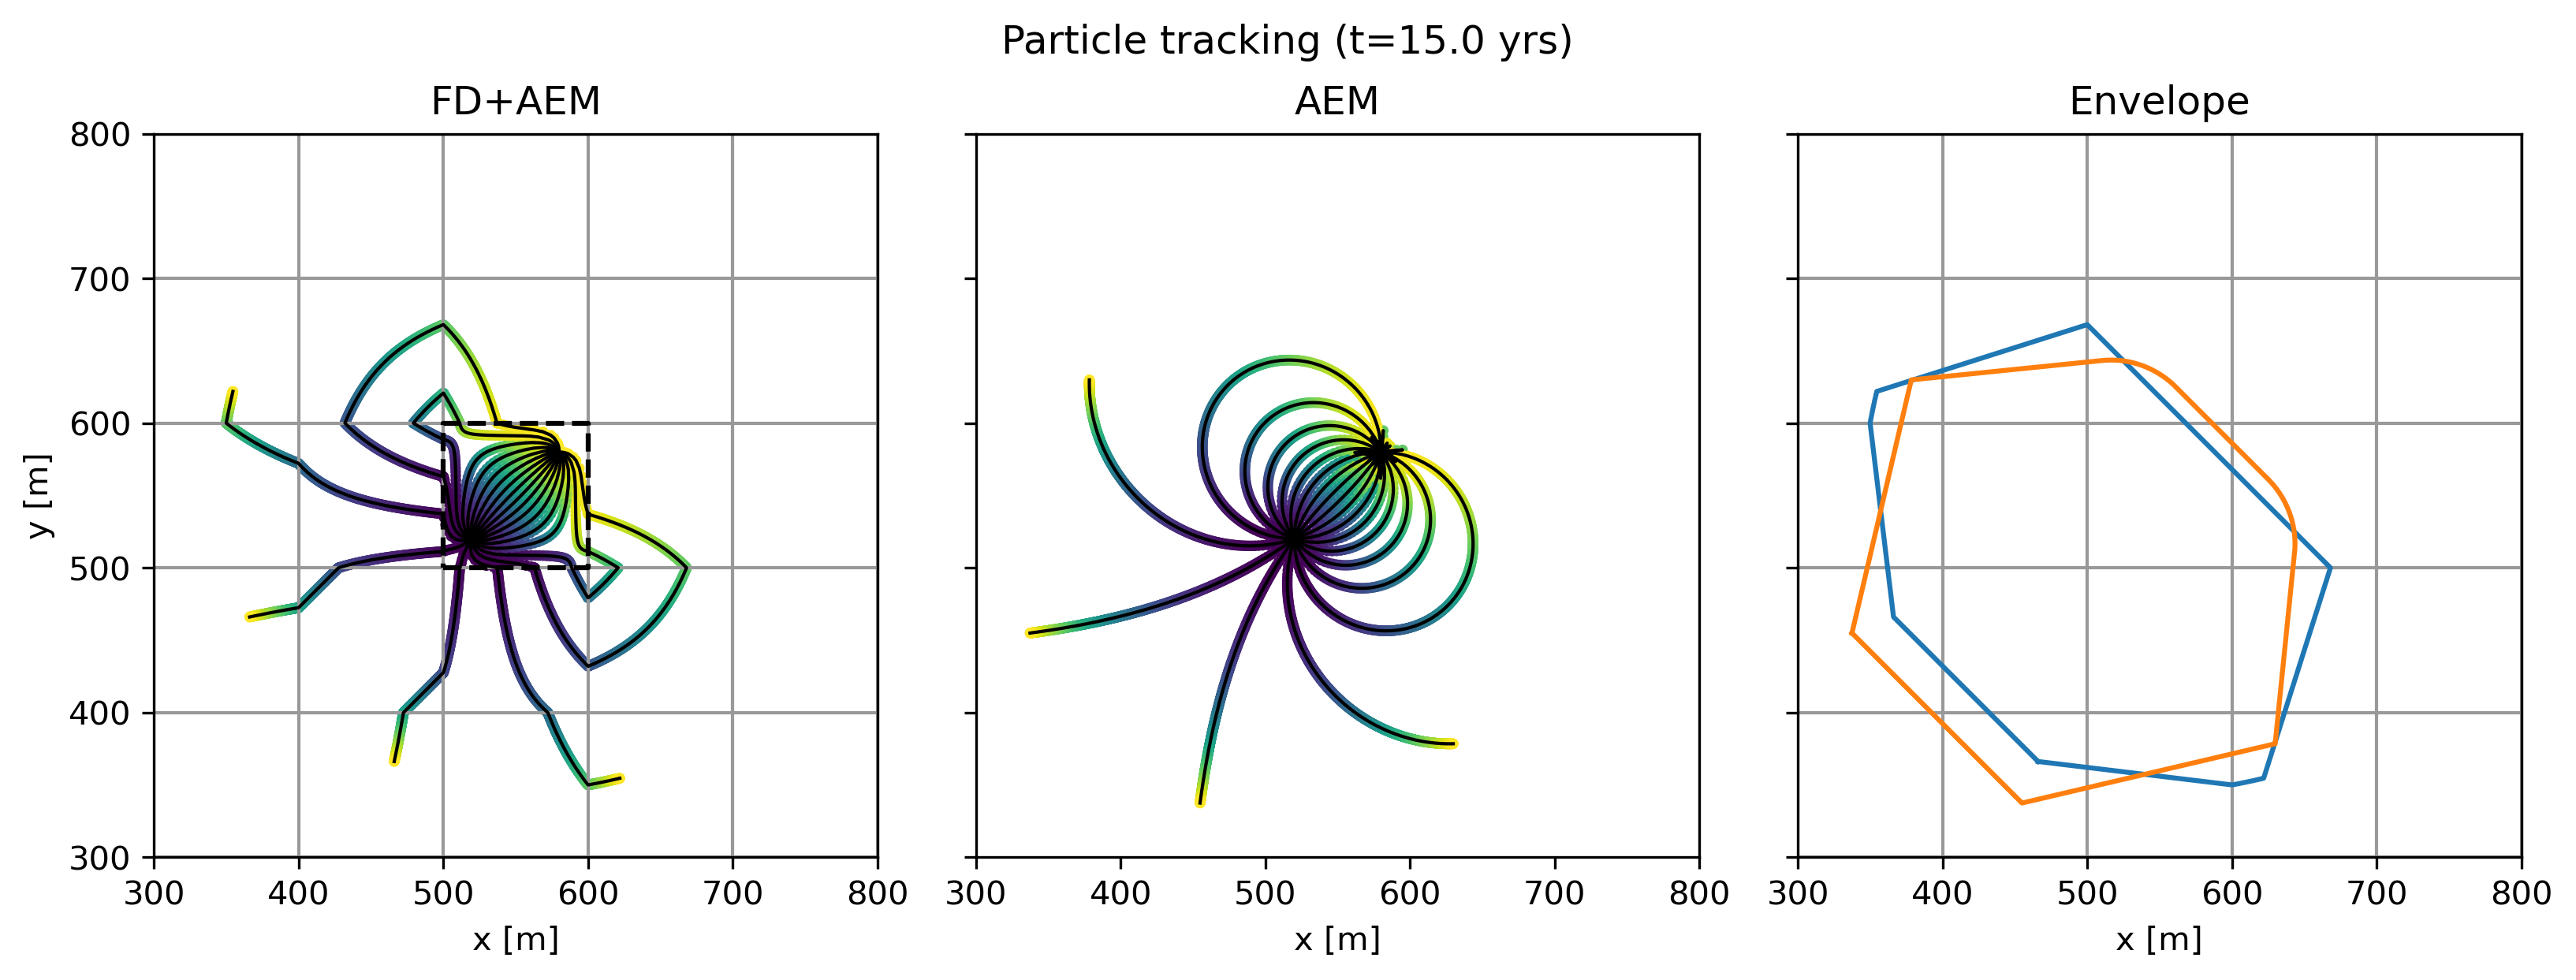
\includegraphics[width=\linewidth]{figures/b05_capture_zone.png}
        \end{tikzfigure}

    }

\end{columns}
\begin{columns}

    \column{0.25}
    \block[bodyverticalshift=-8mm]{Conclusions}{
    \setulcolor{colorBlockTitle}
    \begin{itemize}
        \item AEM has potential as an local refinement method for a FD model. The head and flow can be computed at any point within the AEM cell: \ul{infinite refinement of cell!}
        \item Promising early results coupling FD and AEM models for wells in a single confined aquifer.
        \item General head boundary elements are flexible and satisfy the water balance. Using this element it should be straight-forward to replace multiple FD cells with an AEM model. 
        \item AEM code is written in Python and has an object-oriented structure similar to TimML and TTim. Elements developed in this research can be easily integrated into TimML or TTim.
    \end{itemize}

    % \small
    % \innerblock{Download}{Download poster as pdf: https://bit.ly/IAH2024}
    
    }
    
    \column{0.25}
    \block[bodyverticalshift=-8mm]{Next Steps}{
    \begin{itemize}
        \item Extend solution to semi-confined and transient flow in multi-aquifer systems.
        \item Integrate analytic elements into the TimML/TTim Python packages. 
        \item Replace the top-layer (e.g. drainage system) in a FD model with an AEM model.
        \item Test method on a real-world example, e.g. compute flow around a drinking water production well field.
        \item Couple directly with Modflow 6 using the Modflow API. Create a MF6-AEM package. 
    \end{itemize}

    }    

    \column{0.25}
    \block[bodyverticalshift=-8mm]{References}{
        \nocite{*}     
        
        % \vspace{-5mm}
        \begingroup
        \renewcommand{\section}[2]{}%
        % \scriptsize
        \footnotesize
        \bibliography{references.bib}
        \endgroup
    }

    \column{0.25}
    \block[bodyverticalshift=-8mm]{Link to PDF}{
   
    \vspace{3mm}
    \centering
    
\includegraphics[height=120mm]{figures/bit.ly_IAH2024_FD_AEM.png}
    }
    
    
\end{columns}


    
\node [above left,font=\Huge,outer sep=7.5mm, align=left] at (bottomleft -| topright) {\color{white} \sffamily \Large \emailsymbol d.brakenhoff@artesia-water.nl};


\end{document}